%% thesis.tex 2014/04/11
%
% Based on sample files of unknown authorship.
%
% The Current Maintainer of this work is Paul Vojta.

\documentclass{ucbthesis}
\usepackage[sorting=none]{biblatex}
% \usepackage[backend=bibtex]{biblatex}
\usepackage[english]{babel}
\usepackage{setspace}

\usepackage{amssymb}

%% The amsthm package provides extended theorem environments
\usepackage{amsthm}
\usepackage{epsfig}
% \usepackage{times}
\renewcommand{\ttdefault}{cmtt}
\usepackage{amsmath}
\usepackage{graphicx} % for graphics files

% Draw figures yourself
\usepackage{tikz}

% writing elements
\usepackage[version=3]{mhchem}

% The float package HAS to load before hyperref
\usepackage{float} % for psuedocode formatting
\usepackage{xspace}

% from Denovo Methods Manual
\usepackage{mathrsfs}
\usepackage[mathcal]{euscript}
\usepackage{color}
\usepackage{array}
% \usepackage{hyperref}
% \usepackage[parfill]{parskip}
% \hypersetup{linkcolor=black, citecolor=black, urlcolor=black}
\usepackage{hyperref}
\usepackage{multirow}
\usepackage{notoccite}
\hypersetup{
      colorlinks,
      citecolor=black,
      filecolor=black,
      linkcolor=black,
      urlcolor=black
                    }
%
%
%  Add math definitions
\DeclareMathOperator\erf{erf}


% To compile this file, run "latex thesis", then "biber thesis"
% (or "bibtex thesis", if the output from latex asks for that instead),
% and then "latex thesis" (without the quotes in each case).

% Double spacing, if you want it.  Do not use for the final copy.
% \def\dsp{\def\baselinestretch{2.0}\large\normalsize}
% \dsp

% If the Grad. Division insists that the first paragraph of a section
% be indented (like the others), then include this line:
% \usepackage{indentfirst}

\newtheorem{theorem}{Jibberish}

\bibliography{references}

\hyphenation{mar-gin-al-ia}
\hyphenation{bra-va-do}

\begin{document}

% Declarations for Front Matter

\title{FW/CADIS-$\Omega$: An Angle-Informed Hybrid Method for Neutron Transport}
\author{Madicken Munk}
\degreesemester{Summer}
\degreeyear{2017}
\degree{Doctor of Philosophy}
\chair{Assistant Professor Rachel N. Slaybaugh}
\othermembers{Assistant Professor Massimiliano Fratoni \\
  Professor John Harte \\
  Dr. Tara Pandya}
\numberofmembers{4}
% Previous degrees are no longer to be listed on the title page.
% \prevdegrees{B.A. (University of Northern South Dakota at Hoople) 1978 \\
%   M.S. (Ed's School of Quantum Mechanics and Muffler Repair) 1989}
\field{Nuclear Engineering}
% Designated Emphasis -- this is optional, and rare
% \emphasis{Colloidal Telemetry}
% This is optional, and rare
% \jointinstitution{University of Western Maryland}
% This is optional
\campus{Berkeley}

% For a masters thesis, replace the above \documentclass line with
% \documentclass[masters]{ucbthesis}
% This affects the title and approval pages, which by default calls this
% document a "dissertation", not a "thesis".

\maketitle
% Delete (or comment out) the \approvalpage line for the final version.
\approvalpage
\copyrightpage

% (This file is included by thesis.tex; you do not latex it by itself.)

\begin{abstract}

% The text of the abstract goes here.  If you need to use a \section
% command you will need to use \section*, \subsection*, etc. so that
% you don't get any numbering.  You probably won't be using any of
% these commands in the abstract anyway.

Invasive brag; forbearance.

\end{abstract}


\begin{frontmatter}

\begin{dedication}
\null\vfil
\begin{center}
This dissertation is dedicated to the internet of cats: a series of
interconnected paws, tails, fur, space, and autotune. \\

\vspace{15mm}

Thanks also to the human family, friends, and mentors for the support and
assistance that, sometimes, only opposable thumbs can provide.
\end{center}
\vfil\null
\end{dedication}

% You can delete the \clearpage lines if you don't want these to start on
% separate pages.
\setcounter{secnumdepth}{3}
\setcounter{tocdepth}{3}

\tableofcontents
\clearpage
\listoffigures
\clearpage
\listoftables

% (This file is included by thesis.tex; you do not latex it by itself.)

\begin{acknowledgements}

I have been profoundly lucky to have met and worked with some truly inspiring
people throughout my studies in nuclear engineering. Before I begin, I must say
that I would not be here without the contributions--whether large or small--from
all of these wonderful people. I say this with the deepest sincereity: thank you
to all of you.

First, I must thank my advisor, Prof. Rachel Slaybaugh. Rachel, you saw me through
the highest peaks and deepest valleys of my journey in
graduate school, and you provided
nothing but support and encouragement. Thank you for sincerely caring about my
well-being, facilitating my pursuit of knowledge, and enabling me to
push my myself even when I thought it wasn't possible.
Your mentorship has led to my foray into the world
of hybrid methods,
a field to which I never thought I could contribute. Your technical
knowledge and sincere commitment to your students is unparalleled.

I am immensely grateful for my collaborators at Oak Ridge National Laboratory
for their guidance and support. Without their help and mentorship,
my methods development and
software contributions would be far more paltry. Drs. Tara Pandya, Seth Johnson,
Steven Hamilton, and Tom Evans have all been crucial in my professional
transformation, each in their own way.
Tara, the coolest sparkle-transport-developer in the world, thank you for taking
the time to mentor me and help me to learn a topic which was intitially very
overwhelming. Thank you also for your thorough weekly feedback on this project,
which only made this work stronger.
Seth, I aspire to have even a small fraction of
the astronomical quantity of knowledge of Python, software devleopment, and
software usability in your head. Thank you for helping me learn so much more
about methods development than I thoguht possible.
Steven, your cynicism beyond your years is truly astounding. Thank you for the
math help and absurd humor to brighten my days.

I'd also like to thank my remaining committee members,
Profs. Massimiliano Fratoni and John Harte
for serving on my committee and providing feedback on the work contained in this
dissertation.

I have been fortunate to have many great teachers throughout my young career in
research thus far. Thank you Prof. Rick Norman for being a wonderful mentor and
embodiment of a quality teacher. I also have deep gratitude for my undergraduate
advisor, Dr. Todd Palmer, and mentor, Dr. Steve Reese, who gave me the
opportunity to pursue research as a young and inexperienced undergraduate
student. Their
passion for research, wealth of knowledge, and kidness
influenced my choice to go to graduate school.

My pursuits in graduate school would have been far more difficult had my friends
not kindly supported, encouraged, and helped me in times of need. I am honored
to have such an inspiring group of people that I am able to call my friends.
First, to Denia Djoki\'c, whose kindness knows no bounds and whose imagination is
unparalleled. Denia, I can't believe
that I met you on my first visit to Berkeley so many years ago, and we remain
friends to this day. To Katy Huff, who always has helped me
take pause and consider the deeper impact of my work and whose determination and
achievements are a continuous source inspiration for me.
To Alejandra Jolodosky, my cat-sister for life.
To Ashley Reichardt, who
helps me to see a different perspective every time we talk and who allows
me adventerous escapes from the day-to-day grind.
To Patricia Schuster, my
book club buddy and unwavering cheerleader. To Lakshana, for her
ability to be kind to any person in any circumstance,
even when they talk about her mom or change her background to animals kissing.
And to Kelly Rowland, my
commiserator in-chief. In no particular order,
thank you to my other academic friends: Nathan Bailey,
Sam Briggs, Sandra Bogetic, Tomi Akindele,
Anagha Iynegar, Perry Chodash, James Bevins, Seth Cadell,
and Micah Folsom.
Thanks to my past collaborators on non-dissertation research, in
particular Leah Morgan. Finally, thank you to the fellows and staff at the
Berkeley Institute for Data Science for allowing me to write and work on this
project in a stimulating, coffee-abundant, invigorating place.

Finally, I must thank my nuclear
family for sowing and nurturing my desire for
knowledge, my California family for
ensuring I lived a life outside of graduate
school, and my bay area friends for making the past several years in California
so special.
Last, I'd also like to thank Paul, for his unwavering
support, patience, and kindness. \\ \\

\footnotesize{This material is based on work supported by the Department of Energy under award
number DE- NE0008286. This report was prepared as an account of work sponsored
by an agency of the United States Government. Neither the United States
Government nor any agency thereof, nor any of their employees, makes any
warranty, express or implied, or assumes any legal liability or responsibility
for the accuracy, completeness, or usefulness of any information, apparatus,
product, or process disclosed, or represents that its use would not infringe
privately owned rights. Reference herein to any specific commercial product,
process, or service by trade name, trademark, manufacturer, or otherwise does
not necessarily constitute or imply its endorsement, recommendation, or favoring
by the United States Government or any agency thereof. The views and opinions of
the authors expressed herein do not necessarily state or reflect those of the
United States Government or any agency thereof.}

\end{acknowledgements}


\end{frontmatter}

\pagestyle{headings}

% (Optional) \part{First Part}

\chapter{Introduction}
\label{ch:introduction}

This dissertation covers the development,
implementation, and characterization
of a novel hybrid method for neutral particle, deep-penetration, steady state, radiation transport in
highly anisotropic problems. The method generates a forward-weighted adjoint
scalar flux, which is then used to consistently generate variance reduction
parameters for Monte Carlo radiation transport. Because of the incorporation
of directionality into the adjoint scalar flux,
the method has been named FW/CADIS-$\Omega$. The name alludes to the lineage of
the method, which builds on
the Consistent Adjoint-Driven Importance Sampling (CADIS), and
Forward-Weighted CADIS (FW-CADIS) methods. %need citation
This research both develops a new method that can be used in problems with
strong anisotropies, and also provides a novel
analytical framework by which to characterize anisotropy characteristics of problems. This
work advances the current state of hybrid methods and extends the availability
for different hybrid methods in existing software.


\section{Motivation}
\label{sec:motivation}

Radiation shielding is a realm of continued importance for nuclear engineering,
nuclear security, and health physics applications.
With the expansion of nuclear technology
applications,
the potential proliferation of nuclear materials, and the continued development of
nuclear medicine, tools with which to predict the behavior
of these systems are
in ever-increasing demand. Over the course of many decades, radiation
transport methods have been developed in two primary areas: stochastic (Monte
Carlo) and
deterministic.

These tools have the potential to be immensely
powerful, but are not without their drawbacks. Monte Carlo methods have the
benefit of modeling transport that is continuous in energy, space, and angle.
A user can obtain results for any region in phase-space that one might desire.
However, Monte Carlo methods also require adequate sampling in order to obtain a
solution with sufficient precision. Adequate sampling depends on the number of
particles transported to the tally region. The more particles that are run in a
problem, the
longer the computational time required. Depending on the complexity of the problem,
this may be difficult, computationally demanding, very time consuming,
or impossible.

Deterministic
transport methods discretize the problem phase-space in space, energy, and
angle. They iteratively converge on a global problem solution that is equally
valid across the entire problem space, rather than a potentially localized tally
location. Deterministic solvers tend to be much faster
than Monte Carlo methods, but also lose
the continuity in phase-space that is offered by Monte Carlo. Depending on the
coarseness of the problem discretization,
features of interest in the particle flux may be incorrect, obfuscated,
or missed entirely.

Hybrid methods leverage the speed and uniform solution validity of
deterministically-obtained transport solutions to bias Monte Carlo transport to
more effectively sample in regions of interest. Biasing Monte Carlo to move
particles to regions of interest more effectively
is called variance reduction. Many existing
implementations of hybrid methods
automate the variance reduction process to speed up the time to a
desired solution or to achieve a more uniform uncertainty distribution in the
problem.

Hybrid methods have been designed for an assortment of applications, and none are
universally applicable to all problem types. In particular, hybrid methods are
wanting for a method well-suited for
highly anisotropic, deep-penetration radiation transport applications. The work
presented herein endeavors to provide a potential solution for such applications.

\section{Research Objectives}
\label{sec:objectives}

This dissertation addresses a number of research objectives. The
primary research goal is to:
\begin{itemize}
  \item develop a hybrid method capable of generating variance reduction
    parameters for highly anisotropic, deep-penetration radiation transport problems.
\end{itemize}
Several supporting objectives accompany this goal. They are:
\begin{enumerate}
  \item Propose a hybrid method that capitalizes on a solid theoretical framework
    and lessons learned from existing hybrid methods.
  \item Implement the method in a software package such that it is transparent
    and reproducible.
  \item Devise a rigorous and consistent set of metrics with which to quantify
    method performance.
  \item Develop a suite of problems that have anisotropic behavior induced by
    the problem physics with which to characterize the method.
  \item Run the method and existing hybrid methods on the suite of problems.
    Using the results obtained from these runs, compare the method's
    performance to exiting hybrid methods.
  \item Investigate the sensitivity of the method to other angular-flux
    perturbing parameters, such as the angular discretization of the
    deterministic transport.
\end{enumerate}
By
addressing each of these objectives, the new method will be
proposed, developed, implemented, and characterized such that its behavior in
different problems is well-understood and the method is usable by interested
parties that do not have the expertise of a developer or the author.


% \section{Methodology}
\label{sec:methodology}

In this dissertation, a new hybrid method that incorporates angular information
into the variance reduction parameters it generates is proposed. The method,
named the $\Omega$-method or CADIS-$\Omega$-method, rests on a strong
theoretical basis.

As mentioned in Section \ref{sec:motivation}, there are many flavors of hybrid
method that exist for radiation transport. This hybrid
method has been implemented in the Oak Ridge National Laboratory code suite
Exnihilo and hybrid methods software ADVANTG.



\section{Outline of the Dissertation}
\label{sec:outline}

The next several chapters of this dissertation will cover the relevant
background, the pertinent theoretical basis, and the numerical results that
address the research objectives outlined in Section \ref{sec:objectives}.
Chapter \ref{ch:lit_review} will provide a
comprehensive background on the theoretical basis on which Monte Carlo methods,
deterministic radiation transport, and hybrid methods for radiation shielding
are founded. In so doing, it will provide context for the existing gaps for
generating variance reduction parameters in
highly anisotropic, deep-penetration radiation transport problems. It will also
highlight the most effective hybrid methods that can be applied to
non-anisotropic, deep-penetration radiation transport problems. Building off of
the knowledge presented in Chapter \ref{ch:lit_review},
Chapter \ref{ch:methodology} will provide an overview of the
theoretical basis of the method developed for this project. The theory
presented in this chapter is novel and contributes to the larger body of hybrid
methods research. This chapter will also cover the software used for this
project, and in which ways it was modified to incorporate the novel theory
presented herein. Next, Chapter \ref{ch:charprobs} will present several problems
with which the method is to be characterized. The results from these problems
will inform a parametric angle-informed study, which will also be presented
later in the chapter. Finally, Chapter \ref{ch:conclusion} will draw from the
results presented in Chapter \ref{ch:charprobs} to discuss the performance of
the new method, to summarize what was learned from the method characterization,
and to suggest future paths forward for future hybrid methods research.







\chapter{Literature Review}
The following literature review aims to contextualize the work described in this
dissertation within the realm of hybrid methods for deep-penetration
neutron transport. In doing
so, it will describe pertinent theoretical information that is relevant to this
topic. This will be supplemented by a discussion of the various efforts
to use these methods practically and the degree to which those methods succeeded.
First a brief overview of variance reduction for monte carlo radiation transport
will be described in section \ref{sec:MCvar}.
This will then transition in section \ref{sec:AutomatedVR} into an elaboration
of various efforts to automate variance reduction techniques within monte carlo.
Following that, section \ref{sec:Importance} will introduce the concept of
importance and how that relates to variance reduction. This section will also
focus specifically on how the adjoint solution of the neutron transport equation
relates to importance.
From this point, the chapter will transition
from theory into existing implementations
of variance reduction techniques used in modern software in the nuclear
engineering community. This will begin in \ref{sec:CADIS} with a description of
the consistent, adjoint-driven importance sampling, or CADIS, and
forward-weighted CADIS (FW-CADIS) methods.
The following section, \ref{sec:AngleVR}, will detail the efforts to incorporate
angular information into variance reduction methods for Monte Carlo.
The sections on CADIS, FW-CADIS, and angle-specific variance reduction
techniques will be concluded with with a description of the
various software in which these methods have been implemented and the degree to
which they have been successful.

\section{Monte Carlo Variance Reduction}
\label{sec:MCvar}

Monte Carlo methods for radiation transport are used in the nuclear
engineering community for a wide spectrum of application problems. Without any
variance reduction techniques, Monte Carlo methods aim to emulate
the transport of a particle from birth, through physical interaction, to death
by randomly sampling probabilities particle production, elastic and inelastic
scattering, and absorption for that particle.
This process of transporting a single particle
is repeated millions of times, which is analogous to transporting
millions of particles throughout the problem. When the user achieves a
sufficient
number of particles to sample to reach the desired statistical precision for
the region of interest, the
simulation will be complete. However, this naive approach to simulating each
particle, no matter whether it is likely to contribute to the tallied result,
can be extraordinarily computationally inefficient depending on the problem. A
user could waste time simulating millions of unusable particles and still not
reach the desired statistical precision for the tally. Variance
reduction techniques were developed to address this issue. In general, these
techniques bias the Monte Carlo transport to more effectively
contribute to a particular result, while not fundamentally changing the nature
of the problem being solved.

\subsection{Statistical Background}
\label{subsec:StatBkgnd}

Variance reduction techniques are rooted in statistics, so we will begin our
discussion of variance reduction techniques with a brief primer on the
statistical background relevant to Monte Carlo radiation transport. Sections
\ref{subsubsec:PopStat} through \ref{subsubsec:FOM} are summarized from
\cite{lewis_computational_1984} and \cite{mcnp_manual_v1}.
Monte Carlo
methods transport many randomly sampled
particles, and when those particles reach a region of interest, they are scored
in a tally. The statistical precision of the tally
will reflect the total number of particles that were sampled in- or at- this
region or surface.
The reliability of the answer obtained in this region is then dependent
on the quantity of these particles,
and the amount of time taken to move the particles on
their respective random walks through space to the region.

\subsubsection{Population Statistics}
\label{subsubsec:PopStat}

In radiation transport, one desires to estimate some response in phase-space.
This response is the average behavior of the physical interactions in some
differential phase-space in energy, space, or time. If the probability density
function $f(x)$ for the response is known exactly,
then the response in $dx$ can be calculated exactly by the true
mean, or
\begin{equation}
  \bar{x} = \int_{-\infty}^{\infty} xf(x) dx .
\end{equation}
Rarely $f(x)$ is known
exactly, so instead it is sampled.
Using $N$ randomly sampled particles, the estimate of the true mean value is given as
\begin{equation}
  \hat{x} = \frac{\sum_{i=1}^{N}{x_i}}{N} ,
\end{equation}
where $x_i$ is the i$^{th}$ event. $\hat{x}$ is the sample mean, or the
estimated value of $\bar{x}$
based on the $N$ number of samples that were used to calculate $\hat{x}$. As $N
\rightarrow \infty$, $\hat{x}$ will $\rightarrow \bar{x}$, which is given by the
Strong Law of Large Numbers \cite{mcnp_manual_v1}.
$\hat{x}$ in itself is a useful measure, but determining the spread of values
about $\hat{x}$ is also an important measure. This is called the variance. The
true variance of the distribution is
\begin{equation}
  \sigma^{2}\big( x \big) = \bar{x^2} - \bar{x}^2 ,
\end{equation}
and the standard deviation is the square root of the variance
\begin{equation}
  \sigma\big(x \big) = \big( \bar{x^2} - \bar{x}^2 \big)^{1/2}.
\end{equation}
The variance of the sampled distribution differs, as a finite number of samples
are used to calculate $\bar{x}$ and $\sigma$. The sample variance is defined by:
\begin{equation}
S^{ 2 }=\sum _{ i=1 }^{ N }{ \frac { (x_{ i }-\hat { x } )^{ 2 } }{ N-1 }  }
             \cong \widehat{x^2}-\hat{x}^2 ,
\label{eq:Var}
\end{equation}
where
\begin{equation}
  \widehat{x^2} = \frac{1}{N}\sum_{i=1}^{N} x_i^2 ,
\end{equation}
and the sample standard deviation is given by
\begin{equation}
  S = \big( \widehat{x^2}-\hat{x}^2 \big)^{(1/2)} .
\end{equation}
For \eqref{eq:Var} to hold true, the number of N samples must be large.
$S^2$ is the sample estimate of the true variance, $\sigma^2$. The variance
tells the observer how spread the sampled values are about the mean.
The variance of the estimate of the mean value about $\bar{x}$ is:
\begin{equation}
S^{ 2 }_{ \hat { x }  }=\frac{S^2}{N}.
\label{eq:VarMean}
\end{equation}
From \eqref{eq:VarMean}, one can see that relationship between the sample standard
deviation and the standard error of $\hat{x}$ about $\bar{x}$, which is
\begin{equation}
S_{ \hat { x }  }=\sqrt { \frac { S^{ 2 } }{ N }  } =\frac { S }{ \sqrt { N }}.
\label{eq:VarN}
\end{equation}
$S_{\hat{x}}$ is the standard error of the estimate of the sample mean.
The relative error normalizes the standard error by estimate of the mean
\begin{equation}
R = \frac{S_{ \hat { x }  }}{\hat{x}} .
\label{eq:RelativeErr}
\end{equation}
As a result, $S$, $R$, and $N$ follow the relationship
\begin{equation}
S^2\:\propto\: R^2\:\propto\:\frac{1}{N} .
\label{eq:S to R}
\end{equation}

\subsubsection{The Central Limit Theorem}
\label{subsubsec:CLT}

Suppose that $\hat{x}$ is calculated from several independent random particles
to estimate $\bar{x}$. At what point does one conclude that $\hat{x}$ sufficiently
reflects $\bar{x}$?
The central limit theorem (CLT) \cite{lewis_computational_1984, mcnp_manual_v1}
is a very powerful supplement to the quantities
described in Section \ref{subsubsec:PopStat}. The CLT states that for large N,
$\hat{x}$ will have a limiting distribution $f_N(\hat{x})$, and that distribution will be a
normal distribution
\begin{equation}
  f_N\big(\hat{x}\big) \approx \frac{1}{\sqrt{2\pi} \sigma(\hat{x})}\
           \exp\Bigg[ \frac{-\big( \hat{x}- \bar{x}\big)^2}{2\sigma^2(\hat{x})} \Bigg],\
           \quad N \rightarrow \infty.
  \label{eq:CLT1}
\end{equation}
The standard deviation of $\hat{x}$ can be related to the standard deviation of
the samples by
\begin{equation}
  \sigma(\hat{x}) = \frac{\sigma(x)}{\sqrt{N}}.
\end{equation}
Replacing this in Eq. \eqref{eq:CLT1}
\begin{equation}
  f_N\big(\hat{x}\big) \approx \sqrt{\frac{N}{2*\pi}} \frac{1}{\sigma(x)}\
           \exp\Bigg[ \frac{-N\big( \hat{x}- \bar{x}\big)^2}{2\sigma^2(x)} \Bigg],\
           \quad N \rightarrow \infty
  \label{eq:CLT2}
\end{equation}
allows us to use known values for $\hat{x}$ and an approximation of $\sigma(x)$
using $S$ to determine the probability density function of the sample means
$f_N(\hat{x})$. Because $f_N(\hat{x})$ is a normal distribution, we can find the
probability that $\hat{x}$ lies in $\bar{x} \pm \epsilon$ with
\begin{equation}
  P\big\{\bar{x} - \varepsilon < \hat{x} \leq \bar{x} + \varepsilon\big\} = \
   \int_{\bar{x}-\varepsilon}^{\bar{x}+\varepsilon}f_N\big( \hat{x} \big) d\hat{x}.
   \label{eq:probmean}
\end{equation}
Placing our definition for the distribution of $\hat{x}$ $f_N(\hat{x})$ into Eq.
\eqref{eq:probmean}, changing the limits of integration, and changing the
variables such that $t = \sqrt{N/2}*(\hat{x}-\bar{x})/\sigma(x)$, this becomes
\begin{equation}
  P\big\{\bar{x} - \varepsilon < \hat{x} \leq \bar{x} + \varepsilon\big\} = \
  \frac{2}{\sqrt{\pi}} \int_0^{(\sqrt{N/2})(\varepsilon/\sigma(x))} e^{-t^2} dt
\end{equation}
Recalling the definition of the error function, ends up as
\begin{equation}
  P\big\{\bar{x} - \varepsilon < \hat{x} \leq \bar{x} + \varepsilon\big\} = \
    \erf\Big[\sqrt{\frac{N}{2}} \frac{\varepsilon}{\sigma(x)}\Big].
\end{equation}
Then, using the calculated estimation for $\sigma(x)$ $S$, and also from Eq.
\eqref{eq:VarN} that $S_{\hat{x}}= S/\sqrt{N}$, the error function reduces to be
a function of $\varepsilon$ and $S_{\hat{x}}$ only
\begin{equation}
    \erf\Big[\sqrt{\frac{N}{2}} \frac{\varepsilon}{\sigma(x)}\Big] = \
    \erf\Big[\sqrt{\frac{1}{2}} \frac{\varepsilon}{S_{\hat{x}}}\Big] .
\end{equation}
Should $\varepsilon$ be chosen to be a function of $S_{\hat{x}}$, the error
function reduces further and becomes merely an evaluation as multiples (M), of
$S_{\hat{x}}$ and $\sqrt{1/2}$. For the first few multiples of the standard
error, this is evaluated as
\begin{equation}
  P\big\{\bar{x} - M S_{\hat{x}} < \hat{x} \leq \bar{x} + M S_{\hat{x}} \big\} =
  \begin{cases}
    .683, & M = 1, \\
    .954, & M = 2, \\
    .997, & M = 3
  \end{cases}  .
\end{equation}

The central limit tells us that the sample mean follows a normal
distribution, regardless of the distribution of the underlying sample, as the
number of samples approaches infinity. This
means that no matter what distribution is being sampled, the sampled mean will
have this expected behavior. As a result, given a calculated value for
$\hat{x}$, and $S$, the probability that $\hat{x}$ is near $\bar{x}$ is known
and calculable.
Further, the central limit theorem shows that this distribution is approached
very quickly as N increases, with most problems only requiring $N > 30$
\cite{lewis_computational_1984}. Note
that N is not the total number of samples, but the number of samples required to
calculate each mean.
However, for the central limit theorem to hold a number of
requirements must be satisfied. Ss with all of the quantities in Section
\ref{subsubsec:PopStat}, each $x_i$ is assumed to be randomly sampled and
independent of other $x_i$. If some region of phase space is omitted
accidentally, these values will not be reflective of the true $f(x)$, and so
$\hat{x}$ will not approximate $\bar{x}$. Further, for $S$ to be a
good approximation of $\sigma(x)$, a large number of N samples must contribute
to the calculation of $\hat{x}$. Further, the central limit theorem assumes that
$f(x)$ is a probability density function that can be sampled and has a variance
that exists. As a result, one must be reasonably sure that all of these
requirements are satisfied if using Monte Carlo sampling methods.

\subsubsection{The Figure of Merit}
\label{subsubsec:FOM}

The equations in the preceding sections describe how to estimate the statistics
of a population given a finite number of samples. In radiation transport, a
user seeks to estimate some response, the relative error associated with that
response solution, and time that it takes to obtain those values. Equation
\eqref{eq:S to R} described the relationship between the sample variance, the
relative error, and the number of particles as
\begin{equation*}
S^2\:\propto\: R^2\:\propto\:\frac{1}{N} .
\end{equation*}
The relationship between the relative error $R$ and the number of particles $N$
\begin{equation*}
  R^2\:\propto\:\frac{1}{N}
\end{equation*}
will be some constant value (C)
\begin{equation*}
 C_1 = R^2N .
\end{equation*}
As a problem is simulated, the number of particles run, $N$, will increase
proportionally to the computational transport time run, $T$. Therefore, the
relationship between $R$ and $T$ should also be a constant.
\begin{equation*}
  C_2 = R^2T
\end{equation*}
The figure of merit (FOM) \eqref{eq:FOM}
is the most commonly reported metric that this relationship is reported. It is
widely used in quantifying the effects of variance reduction methods.
Because it uses the inverse quantity of the relative error and time, a
``good'' result would be obtained from a low relative error in a short amount of
time, resulting in a high-value FOM.
\begin{equation}
FOM=\frac { 1 }{ R^{ 2 }T }
\label{eq:FOM}
\end{equation}
Further, a user may desire to determine how long a problem must be run to obtain
a desired relative error. In that case, Equation \eqref{eq:FOM} can simply be
rearranged to
\begin{equation*}
  R = \frac{1}{(FOM*T)^{1/2}} .
\end{equation*}

The figure of merit is a very useful tool that can be used to easily obtain
tally results for a specific problem, but it still is limited by statistical
precision in calculating $R$.
It is worth noting that early on in a transport simulation,
when too few N have been run to
effectively capture $S$ or $\hat{x}$, the Figure of Merit will oscillate.
Eventually it will converge on a relatively constant value. This behavior can
also be used to determine whether one has sufficiently sampled the
region in which they are quantifying the response.

\subsection{Variance Reduction Methods for Monte Carlo Radiation Transport}
\label{subsec:MCVR}
MCNP \cite{hendricks_mcnp_1985, brown_mcnp_2002, mcnp_manual_v1}
has a number of techniques for variance
reduction that are accessible to users. These variance reduction
techniques fall
into four general categories: truncation methods, population control methods, modified
sampling methods, and partially-deterministic methods. Of importance for this
project are
population control methods and modified sampling methods, which are discussed in
a number
of the papers referenced herein. Truncation methods and partially-deterministic
methods do not contribute to and are not the focus of this work,
so will only be touched upon briefly. Note that while this
discussion will tend to focus towards the variance reduction methods in MCNP,
these
methods are by no means limited to this single software package. A
number of other Monte Carlo radiation transport packages also include these
methods.

Population control methods adjust the particle population in the problem to
obtain better sampling in regions of interest by preferentially increasing or
decreasing the particle population.
The first two types of population control methods that will be discussed
are called splitting and rouletting.
Splitting is a method by which the particle population can be increased by
splitting a single higher-weight particle into several lower-weight particles.
Rouletting, conversely, reduces the particle population by stochastically
killing particles. Particles that survive a rouletting routine have their weight
adjusted higher, thereby conserving weight in the routine.
Both splitting and roulette maintain a
fair game by adjusting the particle weights as splitting and rouletting are
performed; the sum of the child particle weights is the same as the parent
weight as it entered the routine.
To use population control methods effectively as a variance reduction technique,
splitting is performed in high-importance regions to increase the particle
count, and thus the sampling, in important regions. Conversely, roulette is
performed in
 low-importance
  regions to reduce the particle population in regions that are unimportant to
  the tally result.
Splitting and roulette can be applied to include geometry, energy and time,
  as well as a weight cutoff.

Rouletting and splitting can be combined in a
single method, generally referred to as weight windows. Figure \ref{fig:ww-mcnp}
illustrates the different processes a particle may go through when entering a
weight window.
%
\begin{figure}
  \centering
  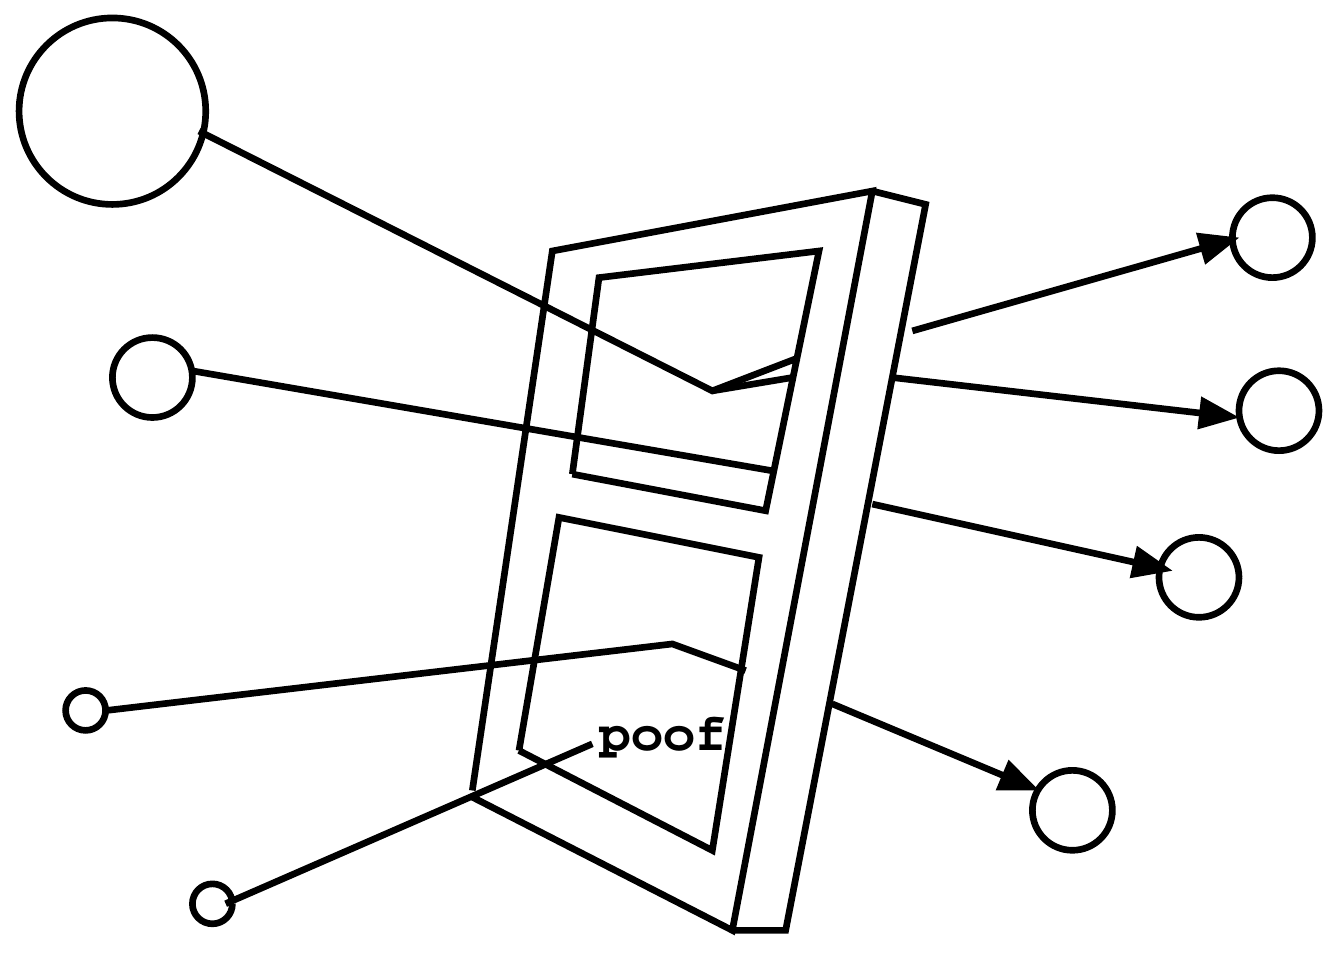
\includegraphics[width=0.5\textwidth]{./chapters/lit_review/figures/ww-mcnp.png}
  \caption[Weight window illustration]{Cartoon illustration of a weight window,
    adapted from \cite{brown_mcnp_2002, mcnp_manual_v2}}
  \label{fig:ww-mcnp}
\end{figure}
%
The first particle we see entering the weight window is a single, high-weight
particle. The weight of this particle is above the weight window bounds, so as
it enters the weight window it is split into multiple particles whose weight is
within the window bounds. The second particle entering the window is within the
weight window bounds, so it retains its weight and is not split or rouletted.
The last two particles entering the window have weights lower than the bound.
They undergo a rouletting routine and one particle is killed and the surviving
particle is increased in weight. As these particles leave the window, all of
them have weights within the range of the window. This will reduce the variance
of the particles contributing to a tally in that region. However, the user is
faced with calculating a significant number of parameters to
determine weight windows for the entire problem. In the best case with an
experienced user, this may just take time. With an inexperienced user or a
difficult problem this can
be insurmountable, and may be too difficult to do without some automated
assistance.

It should be noted that
while splitting and roulette can be performed on a single variable--energy,
space, or time--the weight window is either energy-space
dependent or space-time dependent. Further, the weight window will split or
roulette depending on the particle weight entering the window. Splitting and
roulette on their own either increase or decrease the particle weight
proportional to $I'/I$ no matter what the entering particle weight is. As a
result, poorly chosen splitting or roulette parameters on their own can still
have significant tally variance, because particle weights may still span a wide
range.

Modified sampling methods adjust transport by sampling from a different probability
distribution function than the actual distribution for the problem. This is
possible if, as with population control methods, the particle weights are adjusted
 accordingly.
 The new probability distribution function should bias particles in regions of high
 importance to the problem tallies. In MCNP, a number of modified sampling
 methods exist.
 These include the exponential transform, implicit capture, forced collisions, source
 biasing, and neutron-induced photon production biasing.

The exponential transform modifies particle transport from the analog problem by
artificially modifying the macroscopic cross section, and thus the
distrance-to-collision, to move particles in important directions. In directions
of higher importance, the cross section is reduced, and particles can flow more
freely. In directions of lower importance, the cross section is increased, and
particles more frequently interact, thereby increasing their probability of
directional change or absorption. The transformed cross section used by the
exponential transform is defined by
%
\begin{equation*}
  \Sigma_t^* = \Sigma_t(1-p\mu) ,
\end{equation*}
%
where $\Sigma_t^*$ is the transformed total cross section, $\Sigma_t$ is the
true total cross section, $p$ is the transform parameter, and $\mu$ is the
cosine of the angle between the preferred direction and the particle's transport
direction \cite{mcnp_manual_v1, mcnp_manual_v2, hendricks_mcnp_1985}.

Because the particle's transport is adjusted in the exponential transform, the
particle weight must be adjusted accordingly. This is given by
%
\begin{equation*}
  \begin{split}
  w^* &= \frac{\Sigma_t e^{-\Sigma_t s}}{\Sigma_t^* e^{-\Sigma_t^* s}} \\
      &= \frac{e^{-\rho \Sigma_t \mu s}}{1-p\mu}, \\
  \end{split}
\end{equation*}
%
where $s$ is the phase space of particle residence. This weight adjustment
ensures that the particle weight is conserved throughout transport, even as
the cross section is altered. Because the cross section in the problem is both
energy and material dependent (depending on the geometry), the exponential
transform will be dependent on space and energy, and particles will be biased in
both. While a powerful method, the exponential transform is quite difficult to
use and if $p$ is chosen poorly, this method can perform quite poorly. Further,
the user has to know quite a bit about the problem physics and material to choose an
optimal quantity for $p$.

Source biasing, rather than preferentially adjusting particles' directionality
by way of adjusting the cross sections, biases particles from their origin.
Source biasing has the option to bias particles in energy, direction, and space
(if the source is volumetric). This allows the user to choose importance
separately for each variable. First, the source variable (let us consider
energy for the moment) is defined as a series of bins or a function. Second, the bins are
assigned probabilities of occurence according to their importance. An energy bin
with a high importance will be assigned a high probability of occurence, and a
bin with low importance will be assigned a low probability of occurence. As
particles are born in the bins with higher importances, they will have their
weights adjusted to the inverse of their probability of occurence, or $w^* =
p/p^*$. Here $p$ refers to the probability density function for the source
particles; it bears no relation to the exponential transform factor.

Source biasing is a very simple method that can reduce the solution variance
significantly. However, if a user chooses bin sizes or a function that does not
properly reflect the particles importances in the problem, the source will be
poorly sampled. As a result, sampling may be very inefficient and the figure of
merit will decrease. In MCNP, if poor parameters are chosen for this method, the
user will be given a warning.

Truncation methods stop tracking particles in a region of phase-space that is of
low-importance to the tally. These methods can be used in space (a vacuum boundary
condition), energy (eliminate particles above or below a specified energy), or
time (stop
tracking after a given time). To effectively use these methods, the user must be
aware of
particles' importance to a tally result. If particles that are important to a
result are
 eliminated with a truncation method, the tally will lack the contribution from
 that particle's phase-space, and will be underestimated as a result. Further,
 as discussed in Section \ref{subsubsec:CLT}, the central limit theorem only
 holds assuming that the histories tracked are random and independent.
 Truncating particles of high importance remove the independence from the
 sampling, and the estimate of the response will be wrong.

It is important, in using any variance reduction technique, to ensure that a
fair game
is being played. The user must ensure that the fundamental nature of the problem
is not
being changed by using a variance reduction technique, or the answer will not be
representative of the original problem. Automated variance reduction techniques aim to
eliminate this uncertainty for the user by estimating the importance of
particles in some
 way and then setting up variance reduction parameters automatically.
The remainder of this literature review will focus on efforts to
automate population
control methods and modified sampling methods for variance reduction.

\subsection{Automated Variance Reduction Methods for Monte Carlo Radiation
Transport}
\label{subsec:AutomatedMCVR}

Section \ref{subsec:MCVR} described the methods that one may use to reduce the
variance in Monte Carlo radiation transport tallies. These methods, if used
correctly, can significantly increase the transport efficiency in a Monte Carlo
simulation. However, correct use of these methods often requires intelligent
selection of variance reduction parameters, which is a non-trivial task. Users
found themselves often performing several trial runs before choosing final
quantities for the VR parameters in their problems, which was computationally
inefficient and still required significant knowledge of Monte Carlo and variance
reduction to do well \cite{booth_automatic_1982}.

This has been addressed by using Monte Carlo to sample the problem in an initial
calculation to determine more favorable variance reduction parameters automatically.
Booth and Hendricks,
recognizing that choosing optimal weight window values for energy- and space-
dependent weight windows was difficult even for experienced users proposed a
Monte Carlo importance generator \cite{booth_automatic_1982} that could be used
to select weight window values automatically for a given problem
\cite{hendricks_code-generated_1982}.
The importance generator estimated a cell's importance
by tracking the weights of the particles in the cell, or
\begin{equation}
  Importance  = \frac{\text{score of particles leaving the cell}}
                     {\text{weight leaving the cell}}.
\label{eq:BoothImp}
\end{equation}
and then used these importances to select weight window parameters
\begin{equation}
  W_{i,low} = \frac{1}{kN}\big(\Sigma W_{i,in} + \Sigma W_{i,out} \big)
\end{equation}
\begin{equation}
  W_{i,high} =
  \begin{cases}
    k*W_{i,low} & \text{if } W_{i,low} \neq 0, \\
    \infty & \text{if } W_{i,low} = 0.
  \end{cases}  .
  \label{eq:hendricksWW}
\end{equation}
where $W_{i,low}$ and $W_{i,high}$ are the weight window lower and upper weight
bounds respectively, $W_{i,in}$ and $W_{i,out}$ are the total weight entering
and leaving the cell, $N$ is the number of source particles, and $k$ is some weight
window width (a constant). In his
paper, Booth notes that the weight window target value was chosen so that the
track weight times the expected score in the tally region (for unit track
weight) was approximately constant. Booth's importance generator saw
improvements in the FOM between 1.5-8x when compared to the analog run for the
test problem presented. Booth and Hendricks combined these two methods to
automate weight window generation based on phase-space importance
\cite{booth_deep_1982, booth_importance_1984}. They showed that the combination
of the importance estimator and the weight window generator was a successful way
to perform variance reduction in deep-penetration problems. However, their
method depended on several iterations of importance-determining runs to obtain a
satisfactory estimation of the importance. For a 300cm slab problem, the FOM was
increased from 1.9 to 75, but took 10 subsequent runs to obtain the FOM of 75,
and these runs ranged from 1.2 min (for the analog problem) to 42 minutes (for
the 9th run \cite{booth_importance_1984}.

It should be noted that both the importance generator and the weight window
generator use a lower-quality
Monte Carlo run to gain an initial estimate for a cell's importance and generate
variance reduction parameters from them to bias a more computationally-intensive
run. Naturally, the variance reduction parameters generated by using these
techniques are limited by the statistical precision in the regions used to
generate them. Hendricks also pointed out that the weight window generator
tended to populate all regions of phase space equally, which he conceeded was
not ideal for all problems \cite{hendricks_code-generated_1982}.
Furthermore, for deep-penetration particle transport, the
variance reduction parameters for low flux regions are exceedingly difficult to
generate, resulting in unfavorable VR parameters.

The MCNP \cite{mcnp_manual_v1, brown_mcnp_2002} weight window generator has been
extended beyond the initial space- and energy- implementation described in
booth's paper. It now has the ability to automatically generate space- energy-
and angle- weight windows. The importance generator in MCNP also has been
extended to time-importance, and those values can be used for splitting or
roulette parameters \cite{brown_mcnp_2002}, and can be optimized on a grid
independent from the MCNP geometry \cite{evans_enhanced_1998}.
It As with Booth and Hendricks'
original implementations, this updated weight window generator still relies on
adequate sampling to obtain sufficient weight window parameters. When additional
degrees of freedom, like angle-dependence, are added, this means that the time
to converge on those parameters will take even longer. The weight window
generator also only allows for a single tally to be optimized at once, so
multiple tallies cannot be optimized simultaneously. Last, the weight window
generator still requires user input and updating to seed the weight
window solution. The user must choose the meshing of the problem and have some
intuition as to how the problem should be subdivided. Depending on user
experience, the weight window generator can have differences in the FOM from 2
to 10 times \cite{van_riper_generation_1995}.


\section{Importance Functions for Variance Reduction}
\label{sec:Importance}

The effective use of variance reduction techniques can lead to a faster time to
a desired solution and a reduced variance in the specified tally. However,
specifying variance reduction parameters is not always a straightforward
procedure. In simple geometries, a user might intuitively understand which
regions of a problem may contribute more to a desired solution, but for more
complex geometries, this may not be so obvious.
In the following subsections, the theory in determining which regions of a
problem are important to eliciting a tally response will be described.
The first topic discussed will be
the concept of importance and obtaining a measure of importance with
Monte Carlo sampling.
Second, the adjoint equation and its relation to importance will be introduced.
Last, the contributon solution and how its relation to tally responses is
reviewed.

\subsection{The Concept of Importance}
\label{sec:Importance}

The concept of importance is, in essence, a means of defining which regions of
a problem that are likely to contribute to a
response and which are less likely to contribute to a response. The regions
that are more likely to generate a response will have a
higher importance than those that do not.
If an importance
function for a system can be obtained computationally, that importance
function can be
strategically used in variance reduction techniques to speed up the Monte Carlo
calculations.

As described in Section \ref{subsec:AutomatedMCVR}, Booth
\cite{booth_automatic_1982} proposed
a method to quantify a cell's importance within a Monte Carlo simulation
(Eq. \eqref{eq:BoothImp}). In
this method, Booth suggested estimating the cell's importance using Monte Carlo
transport as:
\begin{equation*}
  Importance  = \frac{\text{score of particles leaving the cell}}
                     {\text{weight leaving the cell}}.
\end{equation*}
This particular calculation of importance
follows from the intuitive explanation for importance in the preceding
paragraph. Recall from Section \ref{subsec:MCVR} that in variance reduction
methods, the population of particles is increased in important regions such that
the number of samples or particles contributing to a tally increases, but the
total problem weight is conserved. More important regions should have many
lower-weight particles to reduce the tally variance. Using Booth's bookkeeping
method for estimating regional importance,
if a cell has a greater weight leaving the cell than the number
of particles, that means that the relative contribution of that cell to the
tally is likely to be lower than other regions. If, instead, the number of
particles leaving the cell is greater than the weight leaving the cell, then
that region is more important to the tally response, because that particle
population is higher than other cells.

While this
estimation of the importance requires only a Monte Carlo forward calculation of
the problem, it was referred to as the forward-adjoint importance generator
\cite{booth_automatic_1982, booth_deep_1982, booth_importance_1984} because the
bookeeping tracked by Eq. \eqref{eq:BoothImp} was a forward-approximation of the
adjoint. Adjoint theory and how it relates to importance will be discussed in
Section
\ref{sec:AdjointImportance}.
Booth's estimation of importance was used to generate
weight window target values inversely proportional to the importance.
In this case, the track weight times the expected score is approximately
constant in the problem. Choosing this inverse relationship between the weight
window and importance is common practice in variance reduction, and is often a
good choice because it is nearly optimal over a broad range of a problem
phase-space \cite{booth_common_2012}.

It should be noted that Booth's method is reliant on the statistical
precision of the cells sampled to generate their importances. For
deep-penetration problems, obtaining a ``good'' estimate of the cell importances
many mean free paths from the forward source takes several iterations. With
large fluctuations between iterations, this has the potential to
be a very slow and
computationally inefficient way to calculate importance in a problem. Using a
solution of the adjoint that is equally valid across all of the problem space
is more ideal for deep-penetration problems.

\subsection{The Adjoint Solution for Importance}
\label{sec:AdjointImportance}

Using the solution of the adjoint formulation of the neutron transport
equation is one of the most widely recognized methods for generating
an importance function. This subsection will begin with a brief summary of
adjoint theory. A discussion on how
the adjoint solution differs physically from the forward solution for a
particular problem follows. Last, some early investigations on how the
adjoint
and importance are related are summarized.

\subsubsection{Theory}

In previous sections we have reviewed the statistical precision of Monte
Carlo-based methods, and how sampled results in Monte Carlo can be obtained
in less time
with variance reduction methods. We have also briefly addressed the forward and
the adjoint solutions for a particular problem. In neutron transport, the
integral form of the forward, steady-state, particle transport equation can be
defined as:
\begin{multline}
\hat\Omega \cdot \nabla \psi
        (\vec {r} ,E,\:\hat\Omega)+\Sigma _{ t }
        (\vec{r},E)\psi (\vec { r } ,E,\:\hat\Omega) = \\
        \int _{ 4\pi  } \int _{ 0 }^{ \infty  } \Sigma _{ s }(E'\rightarrow E,
        \hat\Omega'\rightarrow\hat\Omega)\psi (\vec { r } ,E',\: \hat\Omega')dE'
        \:d\hat\Omega' + q_{e}(\vec { r } ,E, \:\hat\Omega),
\label{eq:F-NTE}
\end{multline}
where $\vec { r }$, $E$, and $\hat\Omega$, are direction, energy, and angle,
respectively, giving six dimensions of phase-space in total.
$\psi$ is the neutron flux, $\Sigma$ is the neutron
interaction (scattering, absorption, total) cross section, and $q_{e}$ is the
external fixed source. Alternatively, this can be written in operator form,
\begin{equation}
  H \psi = q_{e} \:,
\label{eq:F-NTE2}
\end{equation}
where $H$ represents the streaming, scattering, and absorptive terms from Eq.
\eqref{eq:F-NTE}, $\psi$ is the angular flux as it is in Eq. \eqref{eq:F-NTE}, and
$q_{e}$ is the source term.

The forward transport equation tells us where particles are moving
throughout the system. Of note: the
particles move in the scattering term from $E'$ into $E$, and from $\hat\Omega'$
into $\hat\Omega$. Therefore, for a particular problem with a given $q_{e}$,
particles start at $q_e$ and move throughout the system,
either downscattering in energy, streaming out of the problem,
absorbed by the problem materials, or
induce a response at the tally location.

The adjoint equation of the same form, in contrast, can be expressed as:
\begin{multline}
-\hat\Omega \cdot \nabla \psi^{\dagger}
        (\vec {r} ,E,\:\hat\Omega)+\Sigma _{ t }
        (\vec{r},E)\psi^{\dagger}  (\vec { r } ,E,\:\hat\Omega)
       = \\
        \int _{ 4\pi  } \int _{ 0 }^{ \infty  } \Sigma _{ s }(E\rightarrow E',
        \hat\Omega\rightarrow\hat\Omega')\psi^{\dagger}  (\vec { r } ,E',\:
        \hat\Omega')dE' \:d\hat\Omega' + q_{e}^\dagger(\vec { r } ,E,
        \:\hat\Omega),
\label{eq:A-NTE}
\end{multline}
or in operator form as
\begin{equation}
  H^{\dagger} \psi^{\dagger} = q_{e}^{\dagger},
\label{eq:A-NTE2}
\end{equation}
where the variables with $\dagger$ signify the adjoint-specific variables for
the problem: the adjoint flux $\psi^{\dagger}$ and the adjoint source
$q_{e}^{\dagger}$.
Note here that the particles in the adjoint equation move from $E$ into $E'$, and
from $\hat\Omega$ into $\hat\Omega'$, which indicates an upscattering in energy
and a reversal of direction when compared to the forward problem.
The external source, too, is different, changing
from $q_{e}$ to $q_{e}^\dagger$.

To solve the adjoint problem the adjoint source, $q_{e}^{\dagger}$,
can be chosen such that it has the potential to reveal information about the
forward problem. In MC variance reduction, we seek to obtain
information on the
detector or tally response for the system.
The response for the forward problem
given a defined source distribution  $q(\vec{r}, E, \hat{\Omega})$ is
\begin{subequations}
\begin{equation}
  R_{tally} = \int_{4\pi} \int_{V} \int_{E} \psi(\vec{r}, E, \hat{\Omega})
  \Sigma_{tally}(\vec{r},E, \hat\Omega) dE dV d\hat\Omega ,
\end{equation}
where $dE$ $dV$ and $d\Omega$ are the differential spaces of energy, volume, and
angle in the tally region.
This can be simplified using bracket notation, where the brackets indicate an
integration over all phase-space,
\begin{equation}
  R_{tally} = \langle \psi \Sigma_{tally} \rangle .
\end{equation}
\end{subequations}
$\psi$ is the angular flux and $\Sigma_{tally}$ is the effective tally
response function.

For a simple source-detector problem, we choose
$q_{e}^{\dagger}$ to be $\Sigma_{tally}$; or the adjoint source is the
tally/detector response function
for the system. Therefore, the adjoint particles start at low energy at the detector
location, move away from the adjoint source (the detector location), and scatter
up in energy. By making the choice that $q_{e}^{\dagger} = \Sigma_{tally}$, the
response function can be written as a product for the forward flux and the
adjoint source
\begin{equation}
  R_{tally} = \langle \psi q^{\dagger} \rangle .
  \label{eq:response1}
\end{equation}
By using the adjoint identity and the same operators $H$ from Eqs. \eqref{eq:F-NTE2}
and \eqref{eq:A-NTE2}
\begin{equation}
  \langle \psi, H^{\dagger} \psi^{\dagger} \rangle =
  \langle \psi^{\dagger}, H \psi \rangle .
\end{equation}
Eq. \eqref{eq:response1} can be written as a function of the
adjoint flux and the forward source distribution
\begin{equation}
  R = \langle \psi^{\dagger} q \rangle .
  \label{eq:response2}
\end{equation}

At this point, we know that the solution to the adjoint problem
transports particles from the adjoint source (which is the detector or tally
location) into the problem phase-space. The adjoint particles are
upscattered in energy and are transported in $-\Omega$ relative to the forward
problem. However, it may not be immediately obvious how this adjoint solution
relates to importance for the forward solution. Let us start with a simple
illustrative example: a monoenergetic, monodirectional, point source. The
forward source takes the form of a delta function:
\begin{equation*}
  q(\vec{r}, E, \hat{\Omega}) = \delta(\vec{r}-\vec{r}_0) \delta(E-E_0)
  \delta(\hat{\Omega}-\hat{\Omega}_0) .
\end{equation*}
Using this definition of the forward source and evaluating Eq.
\eqref{eq:response2}, we obtain
\begin{equation*}
  \begin{split}
    R &= \langle \psi^{\dagger} q \rangle \\
    &= \int_{V} \int_{E} \int_{\Omega} \psi^{\dagger}(\vec{r}, E, \hat{\Omega})
       q(\vec{r}, E, \hat{\Omega}) d\hat\Omega dE dV \\
       & = \psi^{\dagger}(\vec{r}_0, E_0, \hat{\Omega}_0).
\end{split}
\end{equation*}

This result shows that the solution to the adjoint equation is the detector
response for the forward problem. As a result, the adjoint flux can be used as
an indicator of a particle produced in $\vec{r}, E, \hat{\Omega}$ contributing
to a response in the system. This indicator can be thought of as the particle's
importance to achieving the tally or response objective. Consequently, it is
often said that the adjoint is the importance function for the problem.

The adjoint solution is used in nuclear engineering for a number of
applications, including reactor physics and perturbation theory
\cite{lewins_importance_1965, lewins_developments_1968,
greenspan_developments_1976, lux_monte_1991}.
However, Goertzel and Kalos' early work recognized its
application for deep-penetration radiation shielding.
Goertzel and Kalos \cite{goertzel_monte_1958}
showed analytically
that the exact adjoint solution, if used as an importance or weighting
function for the forward Monte Carlo calculation, will result in a zero variance
solution for the forward Monte Carlo problem. Further, Kalos
\cite{kalos_importance_1963} showed in a 1D infinite hydrogen slab problem that
an analytically-derived adjoint importance function significantly improved the
speed to convergence for neutron
transport in deep-penetration problems.

Goertzel and Kalos' finding that an exact adjoint can lead to a zero variance
solution means that if a single particle is transported with the adjoint
weighting function, its score will be the same as the total system response.
Only a single particle is required to get an exact solution for the forward
problem. This is prohibitive because obtaining
an exact adjoint solution is just as computationally expensive as getting
an exact forward solution. Instead, one seeks to obtain a good, but fairly
inexpensive, estimate of the
adjoint solution based on computational limitations. A good importance estimate
should help reduce the variance in a reasonable amount of time and be
relatively computationally inexpensive. A Monte Carlo solution can
provide a continuous solution over the problem phase-space. However, as
discussed in Section \ref{subsec:MCVR}, the quality of this adjoint solution
relies on the number of samples used to calculate it and that may take a
significant amount of time. A deterministic solution
has the potential to offer equal or better solution confidence across the
entire problem. However, it is discretized in space, energy, and angle.
For deep-penetration importance functions, we
opt for deterministically-obtained solutions due to the solution's equally
distributed validity.

\subsubsection{Implementation}

Coveyou, Cain, and Yost \cite{coveyou_adjoint_1967} expanded on Goertzel and
Kalos' work by interpreting in which ways the adjoint solution could be adapted
for Monte Carlo variance reduction. In particular, they investigated the choice
of biasing schemes and how effective they were at variance reduction for a
simple one-dimensional problem. They reiterated that the adjoint solution is a
good estimate for importance, but should not be calculated explicitly, and
rather estimated by a simpler model. The adjoint function is not necessarily the
most optimal importance function; however, it is likely the closest and most
obtainable estimate of importance that can be calculated
\cite{coveyou_adjoint_1967}. They
concluded that source biasing by the solution to the adjoint equation or by the
expected response is the best choice for Monte Carlo variance reduction, as it
can be used independently from any other variance reduction technique, and
provides good results.

Tang and Hoffman \cite{tang_monte_1988} built off of the parameters derived by
Coveyou et al.\ \cite{coveyou_adjoint_1967} to generate variance reduction
parameters automatically for fuel cask dose rate analyses. In their work, Tang
and Hoffman used the 1D discrete ordinates code XSDRNPM-S to
calculate the adjoint fluxes for their shielding problems. The results from this
calculation were then used to generate biasing parameters for Monte Carlo;
specifically, they aimed at generating parameters for energy biasing, source
biasing, Russian roulette and splitting, and next event estimation
probabilities. They implemented their work in the SAS4 module in SCALE
\cite{SCALE6_1}; it was
one of the earlier implementations of a fully-automated deterministic
biasing procedure for Monte Carlo.

\subsection{The Contributon Solution for Importance}
\label{sec:ContributonImportance}

Contributon theory is another useful concept that can be used as a measure of
importance
\cite{williams_generalized_1991,williams_contributorn_1992,williams_contributon_study}.
However, contributon theory quantifies importance differently than
adjoint theory. In contributon transport, a pseudo-particle, the
\textit{contributon}, is defined. The contributon carries response in the problem
system from the radiation source to a detector. The
total number of contributons in a system are conserved by the \textit{contributon
conservation principle}: all contributons that are emitted from the source
eventually arrive at the detector. Much of the work in this realm has been done
by Williams and collaborators
\cite{williams_generalized_1991,williams_contributorn_1992,williams_contributon_study}.

The contributon transport equation can be derived in a form analogous
to the forward (Eq. \eqref{eq:F-NTE}) and adjoint (Eq. \eqref{eq:A-NTE}) equations.
The derivation of Eq. \eqref{eq:Cont-NTE} and its corresponding variables is
available in a number of the sources referenced in this section, so we will
abstain from re-deriving it here. The angular contributon flux is defined
as the product of the forward and
adjoint angular fluxes:
\begin{equation}
\Psi (\vec {r} ,E,\:\hat\Omega) = \psi^{\dagger} (\vec {r} ,E,\:\hat\Omega)
        \psi(\vec {r} ,E,\:\hat\Omega) \:.
\label{eq.Cont-Flux}
\end{equation}
The contributon transport equation is:
\begin{multline}
\hat\Omega \cdot \nabla \Psi (\vec {r} ,E,\:\hat\Omega)
+\widetilde{\Sigma} _{ t }(\vec{r},E,\:\hat\Omega)\Psi (\vec { r } ,E,\:\hat\Omega)
     = \\
        \int _{ 4\pi  } \int _{ 0 }^{ \infty  }
        \widetilde{p}(\vec{r}, \hat\Omega'\rightarrow\hat\Omega, E'\rightarrow E)
        \widetilde{P}(\vec{r}, \hat\Omega',E')
        \widetilde{\Sigma} _{ t }(\vec{r}, E', \hat\Omega')
        \Psi (\vec { r } ,E',\: \hat\Omega')dE' \:d\hat\Omega'
        + \hat p(\vec { r } ,E, \:\hat\Omega) R .
\label{eq:Cont-NTE}
\end{multline}
The units of phase-space are the same as observed in the forward and adjoint
transport equations. The symbols decorated with tildes denote variables that are
unique to the contributon equation; $\widetilde{p}$ and $\widetilde{P}$ are both
probability functions related to scattering and $\widetilde{\Sigma}$ are
effective cross sections.
The effective cross sections are given by:
\begin{equation}
\begin{aligned}
\widetilde{\Sigma}_{t}(\vec{r}, E, \hat\Omega) &=
        \widetilde{\Sigma}_{s}(\vec{r}, E, \hat\Omega) +
        \widetilde{\Sigma}_{a}(\vec{r}, E, \hat\Omega)    \\
     &= \frac{\iint \Sigma_{s}(\vec{r},\hat\Omega''\cdot\hat\Omega,
         E\rightarrow E'') \psi^{\dagger}
         (\vec{r}, \Omega'', E'') d\Omega'' dE''}
         {\psi^{\dagger}(\vec{r}, E, \hat\Omega)}
        + \frac{Q^{\dagger}(\vec{r}, E, \hat\Omega)}
        {\psi^{\dagger}(\vec{r}, E, \hat\Omega)}.
\end{aligned}
\end{equation}
Note here that the effective scattering and absorption cross sections are
adjoint flux-dependent. Where the adjoint flux becomes small, the interaction
probabilities will become large. As a result, regions where the adjoint flux
is high interaction probabilities become low, causing fewer interactions and
more streaming. Conversely, regions with low adjoint
fluxes--like the problem boundary--will have a very high cross section, thus
encouraging particle transport back towards the adjoint source. This
increased probability of interaction in low flux regions encourages response
particle (contributon)
transport towards the detector or tally, thus contributing to a response.

The scattering probability of a contributon at position $\vec{r}$, $E'$, and
$\hat\Omega'$ is:
\begin{equation}
\widetilde{P}(\vec{r}, \hat\Omega',E') =
         \frac{\widetilde{\Sigma}_{ s }(\vec{r}, E', \hat\Omega')}
       {\widetilde{\Sigma}_{ t }(\vec{r}, E', \hat\Omega')} \:,
\end{equation}
and the probability that a contributon scattering at $\vec{r}$, $E'$,
and $\hat\Omega'$ will scatter into $d\hat\Omega$ $dE$ is
\begin{equation}
\widetilde{p}(\vec{r}, \hat\Omega'\rightarrow\hat\Omega, E' \rightarrow E) =
       \frac{\Sigma_{s}(\vec{r}, \hat\Omega'\cdot\hat\Omega, E'\rightarrow E)
       \psi^{\dagger} (\vec{r}, E, \hat\Omega)}
       {\iint \Sigma_{s}(\vec{r},\hat\Omega'\cdot\hat\Omega'',E'\rightarrow
       E'')\psi^{\dagger} (\vec{r}, E'', \hat\Omega'')d\hat\Omega'' dE''}.
\end{equation}
The distribution function governing the contributon source is
\begin{equation}
\hat p(\vec{r}, E, \hat\Omega) =
\frac{\psi^{\dagger}(\vec{r}, E, \hat\Omega) Q(\vec{r},E,\hat\Omega)}
     {\int \int \int \psi^{\dagger}(\vec{r'},E',\hat\Omega')
     Q(\vec{r'},E',\hat\Omega') d\hat\Omega' dE' dV'},
\end{equation}
note that the contributon source is actually defined in Eq.
\eqref{eq:Cont-NTE} by the product of $\hat{p}$
and $R$. $R$ is contributon production rate; it
is given by integral of the adjoint flux and the forward source
\begin{equation}
  \begin{split}
R &= \int \int \int \psi^{\dagger}(\vec{r},E,\hat\Omega)Q(\vec{r},E,\hat\Omega)
    d\hat\Omega dE dV \\
  & = \langle \psi^{\dagger}Q  \rangle
\end{split} \:,
\end{equation}
which is recognizable as the system response described
in Section \ref{sec:AdjointImportance}. It can also be shown by integrating Eq.
\eqref{eq:Cont-NTE} over all phase space and ensuring that the function
$\hat{p}$ is normalized, that
\begin{equation}
  R = \langle \widetilde{\Sigma}_a \Psi \rangle,
  \label{eq:contribprod}
\end{equation}
or the rate at which contributons die in the detector is the same as
the rate at which they are produced by the contributon source.
Knowing that $R$ is the contributon production rate, let us consider the
probability that a particle will be absorbed in the detector, or $P$, given by
\begin{equation}
  P  = \langle \Sigma_a \psi \rangle.
\end{equation}
Adding a factor of $\psi^{\dagger}/\psi^{\dagger}$ to the terms on the right hand
side, this becomes
\begin{equation}
  P = \Big \langle \frac{\Sigma_a}{\psi^{\dagger}} \psi \psi^{\dagger} \Big
  \rangle.
\end{equation}
By using the identities from the contributon equation, this is also
\begin{equation}
  P = \langle \widetilde{\Sigma_a} \Psi \rangle .
\end{equation}
Next, substituting the definition from Eq. \eqref{eq:contribprod} into this
equation, it follows that
\begin{equation}
  P = R.
  \label{eq:PR}
\end{equation}
This is the same
\textit{contributon conservation principle} introduced at the beginning of this
section.
Williams noted that one could
go so far as to transport contributons rather than real particles with Monte Carlo.
Because every particle transported would eventually reach the detector and give
an exact value for R (as shown by Eq. \eqref{eq:PR}), this
would lead to a zero variance solution. However, the nature of solving the
contributon equation with Monte Carlo (or any other transport mechanism)
involves knowing the exact solution to the adjoint equation, and so relies on
the same computational obstacles as solving the adjoint transport equation.

As mentioned in the previous section, the adjoint flux is an indicator of a
particle's importance to inducing a response. Conversely, the contributon
flux describes the importance of a particle to the solution.
Becker's thesis \cite{becker_hybrid_2009} aptly points out that this is
illustrated most dramatically in a source-detector problem, where the forward
source has little importance to the adjoint source, but does have importance to
the problem solution. As a result, both the contributon solution and the adjoint
solution can be considered importance functions for a problem, but the
importance that they describe differs.

Williams recognized the applications of contributons to
shield design and optimization in an extension of contribution theory called
spatial channel theory. In particular, Williams noted that variables
relevant to contributon response were useful in determining transport paths
through media \cite{williams_contributon_study, williams_SCC_shielding}. A study
of different contributon values throughout the system could enlighten users on
regions with higher response potential. This could then be used to intelligently
choose regions for detector locations or add to shielding.
The contributon values in this theory include the contributon flux, the
contributon density, the contributon current, or the contributon velocity
\cite{williams_relations_1977}.
In this way, the
user could find the particles most influential to the response of the system. A
region with high response potential is the most important to a detector tally. The
variables of response described by Williams are the response potential, the
response current, and the response vorticity \cite{williams_contributorn_1992}.

Contributon theory and spatial channel theory have been applied successfully to
shielding analyses \cite{seydaliev_contributon_2008, williams_SCC_shielding} due
to their ability to show particle flow between a source and response effectively.
Williams and Engle showed that
spatial channel theory can be used in reactor shielding analyses.
In their work, they used
contributon currents to determine preferential flow paths through the Fast Flux
Test Facility (FFTF) \cite{williams_SCC_shielding}.
Seydaliev \cite{seydaliev_contributon_2008} used angle-dependent forward and
adjoint
fluxes and currents to visualize the contributon flux for
simple source-detector problems. In this work, he showed that contributon flow
in the system behaves much like a fluid between the source and detector,
following preferential flow paths more densely.
Seydaliev also observed ray effects in the
contributon flux for high energy photons, and traditional methods like using a
first collision source, did not remedy the issue. The contributon formulation of
particle transport can show important particle flow paths between a source and a
detector, but it is still not immune to computational obstacles that exist for
standard forward- and adjoint- transport.

The past few subsections have described the different means by which importance
can be defined or quantified for a problem.
As discussed in Section \ref{sec:Importance}, generating an importance function
with Monte Carlo is limited in that the quality of the importance map is only as
good as the regions that are sampled. For deep-penetration problems, it may be
prohibitively difficult to obtain adequate importance sampling with traditional
Monte Carlo methods.

Deterministically-obtained importance functions, however,
offer the benefit of a solution that is equally valid across all of the problem
solution-space. This is because the deterministic solution's precision is
limited to convergence criteria, not sampling of individual particles. Using a
deterministic solution is often faster and much less computationally-intensive
than Monte Carlo for importance quantification.
As a result, many hybrid methods opt
to use deterministically-obtained importance functions to generate variance
reduction parameters for Monte Carlo transport.

\section{Automated Variance Reduction Methods for Local Solutions}
\label{sec:localVR}

The next several sections (\ref{sec:localVR} through \ref{sec:AngleVR})
describe different ways that deterministically-obtained importance
functions
can be applied to variance reduction methods in practice. Local variance
reduction methods are those that optimize a tally response in a localized region
of the problem phase-space. These types of problems may be the most immediately
physically intuitive to a user,
where a person standing $x$ meters away from a source may wish to know their
personal dose rate. In this section, notable
automated deterministically-driven variance reduction methods that
have been designed for such localized response optimization are described.
Recall that Booth's importance generator (Section \ref{subsec:AutomatedMCVR})
was also designed for localized tally results, but will not be elaborated upon
here.

\subsection{CADIS}
\label{sec:CADIS}

In 1997, Haghighat and Wagner introduced the Consistent Adjoint-Driven
Importance Sampling method (CADIS)
\cite{wagner_automatic_1997,wagner_automated_1998,haghighat_monte_2003} as a
tool for automatic variance reduction for local tallies in Monte Carlo. CADIS
was unique in that it used the adjoint solution from a deterministic simulation to
consistently bias the particle distribution and particle weights. Earlier
methods had not ensured the consistency between source biasing and particle
birth weights. CADIS was applied to a large number of application problems and
performed well in reducing the variance for local tallies
\cite{wagner_review_2011}.

The next several paragraphs present and discuss
the theory supporting CADIS. Note that the theory presented is specific to
space-energy CADIS, which is what is currently implemented in existing software.
The original CADIS equations
are based on space and energy ($\vec{r}, E$) dependence, but not angle, so
$\phi^{\dagger}$ can be used rather than $\psi^{\dagger}$. This does not mean
that CADIS is not applicable to angle. This is merely a choice made by the
software and method developers given the computational resources
required to calculate and store
full angular flux datasets, and the inefficiency that using angular fluxes might
pose for problems where angle dependence is not paramount.

In trying to reduce the variance for a local tally, we aim to encourage particle
movement towards the tally or detector location. In other words, we seek to
encourage particles to induce a detector response while discouraging them from
moving through unimportant regions in the problem.
Recall from  Eqs. \eqref{eq:response1} and \eqref{eq:response2} that the total
system response can be expressed as either an integral of $\psi^{\dagger}\: q_{e}$
(the adjoint flux and the forward source), or $\psi\: q_{e}^{\dagger}$
(the forward flux and the adjoint source).
Also recall that the adjoint solution is a measure for
response importance.

\begin{subequations}
\label{CADISmethod}
To generate the biased source distribution for the Monte Carlo calculation,
$\hat{q}$,
should be related to its contribution to inducing a response in the tally or
detector. It follows, then, that the biased source distribution is the ratio of
the contribution of a cell to a tally response to the tally response induced
from the entire problem. Thus, the biased source distribution for CADIS
is a function of the adjoint scalar
flux and the forward source distribtion $q$ in region $\vec{r}, E$,
and the total response $R$
\begin{equation}
\begin{split}
\hat{q}  & = \frac{\phi^{\dagger}(\vec {r} ,E)q(\vec {r}
,E)}{\iint\phi^{\dagger}(\vec {r} ,E)q(\vec {r} ,E) dE d\vec{r}} \\
         & = \frac{\phi^{\dagger}(\vec {r} ,E)q(\vec {r} ,E)}{R}.
\end{split}
\label{eq:weightedsource}
\end{equation}
The  starting weights of the particles sampled from the biased source
distribution ($\hat{q}$) must be adjusted to account for the biased source
distribution. As a result, the starting weights
are a function of the biased source distribution and the
original forward source distribution:
\begin{equation}
\begin{split}
w_0  & = \frac{q}{\hat{q}} \\
     & = \frac{R}{\phi^{\dagger}(\vec {r} ,E)}.
\end{split}
\label{eq:startingweight}
\end{equation}
Note that when Eq. \eqref{eq:weightedsource} is placed into Eq.
\eqref{eq:startingweight}, the starting weight is a function of the total
problem response and the adjoint scalar flux in $\vec{r}, E$.
The target weights for the biased particles are given by
\begin{equation}
\hat{w} = \frac{R}{\phi^{\dagger}(\vec {r} ,E)},
\label{eq:WW}
\end{equation}
\end{subequations}
where the target weight $\hat{w}$ is also a function of the total response and
the adjoint scalar flux in region $\vec{r}, E$.
The equations for $\hat{w}$ and $w_0$ match; particles are born at the same weight
of the region they are born into. Consequently, the problem limits
excessive splitting
and roulette at the particle births, in addition to consistently biasing the
particle source distribution and weights. This is the ``consistent'' feature of
the CADIS method.

CADIS supports adjoint theory by showing that using the adjoint solution
($\phi^{\dagger}$) for variance reduction parameter generation successfully
improves Monte Carlo calculation runtime. CADIS showed improvements in the FOM
when compared to analog Monte Carlo on the order of $10^2$ to $10^3$,
and on the order of five
when compared to ``expert'' determined or automatically-generated weight
windows \cite{wagner_automated_1998, wagner_automated_2002} for simple shielding
problems. For more complex
shielding problems, improvements in the FOM were on the order of $10^1$
\cite{wagner_automatic_1997, wagner_automated_1998}. Note that CADIS improvement
is dependent on the nature of the problem and that these are merely illustrative
examples.

\subsection{Becker's Local Weight Windows}
\label{sec:beckerlocal}

Becker's work in the mid- 2000s also explored generating biasing parameters for
local source-detector problems \cite{becker_hybrid_2009}. Becker noted that in
traditional weight window generating methods, some estimation of the adjoint
flux is used to bias a forward Monte Carlo calculation. The product of this
weight window biasing and the forward Monte Carlo transport ultimately
distributed particles in the problem similarly to the contributon flux.
In his work, Becker
used a formulation of the contributon flux, as described in Eq.
\eqref{eq.Cont-Flux} to optimize the flux at the forward detector location.
The
relevant equations are given by Eqs. \eqref{eq:beckerconributon} -
\eqref{eq:beckeralpha}.

\begin{subequations}
\label{eq.beckerlocal}
First, the scalar contributon flux $\phi^c$, which is a function of space and energy
is calculated with a product of the deterministically-calculated forward and
adjoint fluxes, where
\begin{equation}
\phi^c(\vec{r},E) = \phi(\vec{r},E) \phi^{\dagger}(\vec{r},E).
\label{eq:beckerconributon}
\end{equation}
This is then integrated over all energy to obtain a spatially-dependent
contributon flux
\begin{equation}
\tilde{\phi^c}(\vec{r}) = C_{norm}\int_0^{\infty } \phi^c(\vec{r},E) dE,
\label{eq:beckerconributonspace}
\end{equation}
where the normalization constant, $C_{norm}$, for a given detector volume,
$V_D$,
is:
\begin{equation}
C_{norm} = \frac{V_D}{\int_{V_D}\int_0^{\infty } \phi^c(\vec{r},E) dE dV}.
\end{equation}
The space- and energy-dependent weight windows are given by:
\begin{equation}
  \bar{w}(\vec{r},E) = \frac{B(\vec{r})}{\phi^{\dagger}(\vec{r},E)}\:,
\label{eq:beckerlocalww}
\end{equation}
where
\begin{equation}
B(\vec{r}) = \alpha(\vec{r}) \tilde{\phi^c}(\vec{r}) + 1 -  \alpha(\vec{r})\:,
\end{equation}
and
\newcommand{\firs}{\cfrac{\tilde{\phi}^c_{max}}{\tilde{\phi}^c(\vec{r})}}
\newcommand{\seco}{\cfrac{\tilde{\phi}^c(\vec{r})}{\tilde{\phi}^c_{max}}}
\begin{equation}
  \alpha (\vec{r}) = \bigg[ 1 + \exp \bigg( \firs - \seco \bigg) \bigg]^{-1} .
  \label{eq:beckeralpha}
\end{equation}
\end{subequations}

Becker found that this methodology compared similarly to CADIS
for local solution variance reduction
for a large challenge problem comprised of nested
cubes. The particle density throughout the problem was similar
between CADIS and Becker's local weight window. The FOMs were also relatively
similar, but were reported only with Monte Carlo calculation runtimes (meaning
that the deterministic runtimes were excluded). Note that
Becker's method requires both a forward and an adjoint
calculation to calculate the contributon fluxes, while CADIS requires only an
adjoint calculation.

\section{Automated Variance Reduction Methods for Global Solutions}
\label{sec:GlobalVR}

The previous section detailed several methods that automate variance reduction for localized tallies. However, for global solutions these methods do not work well. The global tally suffers from a large range in variance across the physical problem space, and the solution is dependent on the flux distribution throughout the problem. Here several methods are described that provide automated variance reduction for global solutions or multiple tallies. 

Cooper and Larsen developed a weight window technique to reduce the variance of Monte Carlo global solutions \cite{cooper_automated_2001}. In their work, Cooper and Larsen utilized a forward solution to the transport equation to generate paramaters for a modified Monte Carlo simulation where the particles are nearly uniformly distributed throughout the problem. By doing so, the variance in the scalar flux remained relatively constant throughout the problem, rather than rising significantly with increasing distance from the forward source. Cooper's "isotropic" weight windows dependent on $\vec{r}$ are given by:
\begin{subequations}
\label{coopers}
\begin{equation}
\bar{ww}(\vec{r}) = \frac{\phi(\vec{r})}{max \phi(\vec{r})}
\end{equation}
\begin{equation}
ww(\vec{r})_{top} = \rho \bar{ww}(\vec{r})
\end{equation}
b, the linearly anisotropic factor, is
\begin{equation}
ww(\vec{r})_{bottom} = \frac{\bar{ww}(\vec{r})}{\rho}
\end{equation}
where $\rho$ is the weight window scaling factor
\end{subequations}

In practice, Cooper's algorithm was to iteratively switch between solving the diffusion equation with transport correctors (eddington factors); a process known as quasidiffusion, and with a Monte Carlo solution. An initial quasidiffusion solution was used to generate weight windows, and then after a time the Monte Carlo solution was used to generate updated eddington factors for the quasidiffusion solution. 

Because Cooper's method depended on Monte Carlo to generate the eddington factors for the quasidiffusion problem, this method was limited by the iterative switch between the quasidiffusion solution and the Monte Carlo solution. The frequency by which this switching happens is entirely up to the user, but may drastically affect the efficiency of the method. Further, Cooper notes that we do not know at what point in time (for which number of particles N) the Monte Carlo solution becomes more accurate than the quasidiffusion solution, which is an important issue in choosing solution parameters. 

Becker's forward Method: \cite{becker_hybrid_2007}

Becker's contributon method: \cite{becker_hybrid_2009}

Van Wijk's method, like CADIS and FW-CADIS, is a variance reduction method designed to operate with little user input \cite{van_wijk_easy_2011}. 
Van Wijk et al. applied their method to a PWR facility and observed a FOM increase by a factor of $>$200. 


The Method of Automatic Generation of Importances by Calculation (MAGIC) is a global variance reduction technique \cite{davis_comparison_2011} proposed by Davis in 2011. 
Rather than using a deterministic solution to obtain an estimate of the forward flux to generate an importance map, the MAGIC method uses an analog monte carlo run with multigroup cross section data and (optionally) a high energy cut-off.
This initial analog run is used to generate initial importance map for a secondary run.
This process iterates until several monte carlo simulations are run and a finalized importance map is generated. 
In their paper, the authors compared three variants of MAGIC to FW-CADIS in ITER fusion energy systems. 
These three variants used different weight window adjustments for importances: weight windows in cells based on existing weight information, weight windows in mesh cells based on flux information, and weight windows in cells based on population density. 
Davis and colleagues concluded that the most effective method for variance reduction in their system was MAGIC's weight window in mesh based on flux information, where FW-CADIS' FOM was 65\% that of MAGIC's. 
The authors did not make it clear how many iterations were required, on average, to generate the finalized weight window map or if the time to iteratively generate importance maps were included in the FOM. 
It is unclear if only the final monte carlo simulation's runtime was used to calculate the FOM. 
Furthermore, the authors did not clearly state how the biasing parameters were calculated, other than that they used flux, population density, or weight information. 


Forward-Weighted CADIS, also developed by Hagighat and Wagner \cite{wagner_forward-weighted_2007,wagner_forward-weighted_2009,wagner_forward-weighted_2010}, utilized Cooper's concept of using a forward deterministic calculation to evenly distribute particles throughout the problem subspace. However, Wagner et al took a different approach: by using a forward deterministic estimate of the flux or desired response as the adjoint source for an adjoint calculation, biasing parameters for global responses could be calculated. The adjoint source for the adjoint calculation thus depends on the desired response for the system. The generic description for the adjoint source is given by Eq. \eqref{adjointsourcesimple} and more specific parameters are given by Eqs. \eqref{FWCadglbaldose}-\eqref{FWCadglobalflux2}: 

\begin{subequations}
\begin{equation}
{ q^{\dagger}} (P)=\frac{\sigma_d(P)}{R}
\end{equation}
\label{eq:adjointsourcesimple}

The adjoint source for the spatially dependent global dose, $\int \phi(\vec{r},E)\sigma_d(\vec{r},E) dE$:
\begin{equation}
{ q^{\dagger} }(\vec { r } ,E)=\frac { \sigma _{ d }(\vec { r } ,E) }{ \int { \sigma _{ d }(\vec { r } ,E)\psi (\vec { r } ,E,) } dE }
\end{equation}
\label{eq:FWCadglobaldose}

The adjoint source for the spatially dependent total flux $\int \phi(\vec{r},E) dE $:
\begin{equation}
{ q^{\dagger} }(\vec { r })=\frac { 1 }{ \int { \phi (\vec { r } ,E) } dE }
\end{equation}
\label{eq:FWCadglobalflux}

The adjoint source for the energy- and spatially- dependent flux $\phi(\vec{r},E)$: 
\begin{equation}
{ q^{\dagger} }(\vec { r } ,E)=\frac { 1 }{\phi (\vec { r } ,E) }
\end{equation}
\label{eq:FWCadglobalflux2}
\end{subequations}

Comparing these methods, \cite{peplow_comparison_2012} 

%
%
%----------------------------------------------------------------------------------------
% While not particularly relevant to the immediate work described in this thesis, the MS-CADIS method used a sophisticated method to generate a variance-reduced source term for 
% photon does in a shutdown system. 

%However, MS-CADIS, like CADIS and FW-CADIS, employs exclusively energy- and space- based variance reduction methods. As a result, it still suffers from similar behaviors as CADIS and FW-CADIS in strongly anisotropic systems. 

%MS-CADIS \cite{ibrahim_multi-step_2014, ibrahim_analysis_2014}

\section{Automated Angle-Informed Variance Reduction Methods}
\label{sec:AngleVR}

In a number of problems, the angular dependence of the flux is significant enough that
biasing by space and energy, but not angle  is not
sufficient. As a result, a subset of hybrid methods were developed to incorporate some
degree of the flux anisotropy in variance reduction parameters. Without explicitly
calculating the angular flux, which is memory- and storage- intensive, methods
attempted to approximate the angular flux using other information more readily
accessible to them. These approaches broadly can be categorized as methods that
bias using population control methods (such as weight windows),
and methods that bias with modified
sampling methods (such as the exponential transform).
Initial approaches
to angular biasing focused on approximating the angular flux, $\psi$,
as a separable
function of the scalar flux and an angle-dependent multiplier.
These approximations of the flux were then used to generate biasing
parameters dependent on angle for highly angular-dependent problems.

\subsection{Angular Biasing with Population Control Methods}

\subsubsection{AVATAR}
\label{subsec:AVATAR}

The AVATAR \cite{van_riper_generation_1995, van_riper_avatarautomatic_1997}
(Automatic Variance and Time of Analysis Reduction) method generates
three-dimensional, space-, energy- and angle-dependent weight windows for Monte
Carlo by
using a relatively course-mesh and few-angle deterministic calculation in
THREEDANT, approximating the angular flux as a function of the scalar flux, and
then subsequently passing those flux values through a postprocessing
code, Justine, to generate
weight windows for MCNP \cite{mcnp_manual_v1}. The AVATAR approach to
determining the angular flux used an approximation of the angular flux based on
the maximum entropy distribution, which will be briefly summarized in the next
few paragraphs.

\subsubsection*{Information Theory}

First, for a given set of discrete values $x_i (i=1,2, \cdots n)$
that are passed to a function, $f(x)$, the expectation value of that function is given
by
\begin{equation}
  \big\langle f(x) \big\rangle = \sum_{i=1}^n p_if(x_i).
\end{equation}
For the probability distribution $p_i = p(x_i)$, $(i=1,2, \cdots n)$ the entropy of
$p$ is defined as
\begin{equation}
  H(p) = - K \Sigma_i p_i \ln p_i .
  \label{eq:entropy}
\end{equation}
where K is a positive constant. A proof that this is indeed the associated
maximal entropy associated with all $p_i$ is given in
\cite{jaynes_information_1957}.
For a continuous probability density function $p(x)$ over the interval I, the
entropy of the continuous function is
\begin{equation}
  H(p) = - K \int_I\ p(x) \ln p(x) dx .
\end{equation}
To maximize either of these distributions, while also maintaining that $\Sigma
p_i = 1$, one can use Lagrangian multipliers $\lambda$ and $\mu$
\begin{equation}
  p_i = e^{-\lambda-\mu f(x_i)} .
\end{equation}
This can be solved using
\begin{subequations}
  \begin{equation}
    \big\langle f(x) \big\rangle = - \frac{\partial}{\partial \mu} \ln Z(\mu)
  \end{equation}
  \begin{equation}
    \lambda = \ln\big[Z(\mu)\big]
  \end{equation}
  where
  \begin{equation}
    Z(\mu) = \Sigma_i e^{-\mu f(x_i)} .
  \end{equation}
\end{subequations}

Jaynes \cite{jaynes_information_1957} showing that the maximum
entropy probability distribution function corresponding to the previous
equations is given by
\begin{equation}
  p_i= \exp \big[ - \big( \lambda_0 + \lambda_1f_1(x_1) + \cdots + \lambda_m f_m(x_i) \
    \big) \big] ,
\end{equation}
and the entropy of this distribution is given by
\begin{equation}
  S_{max} = \lambda_0 + \lambda_1 \big\langle f_1 (x) \big\rangle + \cdots + \
  \lambda_m \big\langle f_m(x) \big\rangle .
\end{equation}

In this case, the constant K from Eq. \eqref{eq:entropy} has been set to 1.
The maximum entropy approach to calculating a probability distribution function
is an attractive option given limited information about that
distribution. This method's power lies in that it
deduces a function given limited information, but does not place too great of an
importance on missing or unwarranted information. Furthermore, a distribution
ascertained from this methodology will encompass all distributions with smaller
entropies that satisfy the same constraints. Thus it provides the most widely
applicable probability distribution function for the system that has been
defined.

Moskalev showed that by using the maximum entropy approach, a distribution function
could be reconstructed from a (truncated) Legendre expansion
\cite{moskalev_reconstruction_1993}. This is particularly
applicable to radiation transport, because often scattering terms are truncated
Legendre expansions. In his application, Moskalev derived a generalized form of
reconstructing a probability distribution from a truncated expansion, where the
true function represented by a Legendre polynomial series
\begin{equation}
  f(L,\mu) = \sum_{l=0}^L -\frac{2l+1}{2} f_l P_l(\mu)
\end{equation}
could be associated with an adjusted function (obtained from maximizing the
entropy of the known values)
\begin{equation}
  \tilde{f}(L,\mu) = \exp \big( \sum_{l=0}^{L} \lambda_l P_l(\mu) \big)
\end{equation}
such that
\begin{equation}
  (f,P_l) = (\tilde{f}, P_l); \quad l = 0, \cdots, L .
\end{equation}
Where $\lambda_l$ are the Lagrange multipliers, $\tilde{f}$ and $f$ are
$\epsilon \phi$, and are assumed to be a function of $\mu$ such that $f(\mu)
\geq 0, \mu \epsilon [-1, 1]$.
These generalized equations were then applied to
group-to-group scattering probability distribution functions, as well as
reconstructing a $L=3$ function. The reconstruction showed agreement except near
the extrema of $\mu$.

Walters and Wareing \cite{walters_nonlinear_1994, walters_accurate_1996} showed
that the angle-dependent source definition for a discrete ordinates transport problem
could be calculated using Moskalev's approach
\cite{moskalev_reconstruction_1993}. In their method, they used this approach to
reconstruct the source distribution of particles in each cell from the source
moments. For standard methods, the source in a cell expanded in Legendre moments is
\begin{equation}
  S_m(x) = S_{m,j}\bigg[ P_0(x) + \frac{S_{m,j}^x}{S_{m,j}}P_1(x)\bigg]
\end{equation}
where $S_{m,j}$ is the average source in cell j, direction m, $S_{m,j}^x$ is the
$P_1(x)$ moment of the source and the $P_0$ and $P_1$ are the associated
Legendre polynomials. Using a normalized source distribution $s_m(x)$ where
\begin{equation*}
  S_m(x) = s_m(x) S_{m,j},
\end{equation*}
the normalized distribution is
\begin{equation}
  s_m(x) = \big[ s_0 + s_1 P_1(x)\big]
\end{equation}
where $s_0$ and $s_1$ are the zeroth and first Legendre moments of the source.
The source distribution derived from the maximum entropy distribution was found
to be
\begin{equation}
  \tilde{s}(x) = \frac{\lambda_{1,k}}{\sinh (\lambda_{1,j})} \
  e^{\lambda_{1,j}P_1(x)} .
\end{equation}
$\tilde{s}$ has normalized Legendre moments $s_0$ and $s_1$ that match
$s_m(x)$. Because $\tilde{s}$ satisfies the information that can be obtained
about $s_m$, it can be used to reconstruct $S_m(x)$ by way of
\begin{equation}
  S_m(x) = \tilde{s}_m(x)S_{m,j}.
\label{eq:Walt_reconstruct}
\end{equation}
$\lambda_{1,j}$ can be found from
\begin{equation}
  s_1 = 3\bigg[ \coth(\lambda_{1,j} - \frac{1}{\lambda_{1,j}})\bigg] .
  \label{eq:WW_lambda}
\end{equation}
It should be noted that the same methodology that Walters and Wareing use to reconstruct the source
distribution from the source moments can be used to reconstruct the angular flux
in cells based on moments of the angular flux (i.e. the scalar flux and
current) \cite{walters_nonlinear_1994}.

In their paper, Walters and Wareing \cite{walters_accurate_1996} suggested that in place of
solving Eq. \eqref{eq:WW_lambda} for $\lambda_{1,j}$, that a rational polynomial
be used in place of it to reduce computational time. The
suggested polynomial for $0 \leq \lambda_{1,j} \leq 5$ was:
\newcommand{\lamvar}{\dfrac{s_{1,j}}{3}}
\begin{equation}
  \lambda_{1,j} =  \dfrac{2.99821 (\lamvar) - 2.2669248 (\lamvar)^2 }{1 - 0.769332
             (\lamvar) -0.519928 (\lamvar)^2 + 0.2691594 (\lamvar)^3} \\
\end{equation}
and for $\lambda \geq 5$:
\begin{equation}
  \lambda_{1,j} = \frac{1}{1-\bar\mu}
\end{equation}
A full derivation of Eq. \eqref{eq:WW_lambda} and how it satisfies the maximum
entropy requirements can be found in Appendix A of \cite{walters_accurate_1996}.

In their application, Walters and Wareing found that this method was accurate
over a fairly course mesh for the problems analyzed, and the computed fluxes
remined positive over the solution space. When compared to other methods, this
approach performed much better over coarse meshes. However, the analysis was
limited to one-dimensional problems. As mesh size grew finer, the method
performed similarly to other methods. However, near vacuum boundary conditions
$\lambda_{1,j} \rightarrow \infty$ at the cell boundary, causing issues in
calculating the flux in these cells.

\subsubsection*{AVATAR Implementation}

AVATAR used a deterministic

AVATAR built off of the methodology described by Walters and Wareing
\cite{walters_nonlinear_1994, walters_accurate_1996}, but instead of
reconstructing the source distribution inside the cell, the maximum entropy
method was used to reconstruct the angular fluxes. Thus the angular flux, $\psi$
was reconstructed with the scalar flux, $\phi$ and the current, $J$.
AVATAR avoided generating explicit angular fluxes with
THREEDANT by assuming
that the adjoint angular flux is symmetric about the average adjoint current vector,
$J^{\dagger}$ :
\begin{subequations}
\label{avatareqns}
\begin{equation}
  \psi^{\dagger}(\hat\Omega) = \psi^{\dagger}(\hat\Omega\cdot n)
  \label{eq:Av1}
\end{equation}
where
\begin{equation}
  n = \frac{J^{\dagger}}{ \left\| J^{\dagger} \right\| }.
\end{equation}
Note that $n, J, \psi,$ and $\phi$ all have implied dependence on $(\vec{r},
E)$.
The angular flux could then be reconstructed assuming that the angular flux is a
product of the scalar flux and some angle-dependent function
\begin{equation}
  \psi^{\dagger}(\hat \Omega \cdot n) = \phi^{\dagger} f(\hat\Omega \cdot n).
  \label{eq:Av2}
\end{equation}
Note that Eq. \eqref{eq:Av2} takes the form of Eq. \eqref{eq:Walt_reconstruct}.
Thus f is derived from the maximum entropy distribution:
\begin{equation}
f(\hat\Omega \cdot n) = \frac{\lambda e^{(\hat\Omega \cdot n)\lambda}}
                             {2 \sinh {\lambda} }
  \label{eq:Av25}
\end{equation}
and $\lambda$ is a function of the average cosine $\bar\mu$
\begin{equation}
\begin{split}
\lambda  & = \frac{2.99821 \bar\mu - 2.2669248 {\bar\mu}^2 }{1 - 0.769332
             \bar\mu -0.519928 {\bar\mu}^2 + 0.2691594 {\bar\mu}^3} \\
         & = \frac{1}{1-\bar\mu} \\
  \label{eq:Av3}
\end{split}
\end{equation}
for $ 0 \le \bar\mu < 0.8001$ and $0.8001 \le \bar\mu < 1.0 $, respectively.
Also, $\mu$ is given by
\begin{equation}
\bar\mu(\vec{r}, E) = \frac{\left\| J^{\dagger}(\vec{r}, E)
                     \right\|}{\phi^{\dagger}(\vec{r}, E)}.
  \label{eq:Av4}
\end{equation}
\label{eq:AvEqns}
\end{subequations}
Equations \eqref{eq:Av3} and \eqref{eq:Av4} are exact in both isotropic and
streaming conditions \cite{van_riper_generation_1995}.

Using the calculation of the angular flux described in Eqs. \eqref{eq:Av1}
through \eqref{eq:Av4}, angle-dependent weight windows could be constructed.
AVATAR's space- energy- and angle-dependent weight window is given by
\begin{equation}
\bar {w} (\vec{r},E,\hat\Omega) = \frac{k}{\phi^{\dagger}(\vec{r},E)
                                  f(\hat\Omega \cdot n)},
\end{equation}
where k is a constant that can be adjusted to match the source distribution.
In the case of AVATAR, k was used as a normalization factor to ensure that
source particles are born with weights within the weight window.
AVATAR exclusively generated weight windows, and did not attempt to consistently
bias the source
distribution. Physically, the assumption behind AVATAR is that the adjoint
angular flux
is locally one-dimensional, so azimuthal symmetry is assumed.

\subsubsection*{AVATAR Results}

The authors of AVATAR showed that AVATAR's angularly-dependent
weight windows improved the FOM (from 5- to 7-times) for a multiple-tally well-logging
problem compared to the MCNP weight window generator. AVATAR was also compared
to other methods in subsequent papers \cite{evans_enhanced_1998}. In an
update of the MCNP weight window generator, AVATAR was compared to variants of
the weight window generator and performed had a FOM of 79 while variants of the
weight window generator had FOMS ranging from 105 to 119
\cite{evans_enhanced_1998}. However, they required
multiple iterations of Monte Carlo transport to converge on weight window values
while AVATAR did not. Total runtimes for iteratively converging on weight window
values were in the 200- to 300- minute range, while AVATAR took roughly 5
minutes to converge on weight window values for the problem.

The MCNP weight window generator has also been adapted to use weight window
values seeded by a solution from AVATAR \cite{evans_enhanced_1998}. This method
had FOMs comparable to the default MCNP weight window generator, but only
required 1 iteration to converge, rather than 3. This reduced the total
transport runtime from roughly 260 minutes to 140 minutes, but still required
user experience and input to adequately set up and prepare the deterministic
input for AVATAR.

The method used by AVATAR to produce angle-dependent weight windows successfully
incorporated angular information into variance reduction parameters for Monte Carlo
with very little additional computational burden. However, because AVATAR
was not fully automated, the user had to have knowledge on the use of the $S_N$
deterministic solver in addition to the Monte Carlo methods they were trying to
optimize. As a result, the user needed to adequately prepare the deterministic
inputs, correctly specify the adjoint source for the deterministic solve, and
then pass these values to postprocessing software \cite{peplow_consistent_2012,
evans_enhanced_1998}. The FOMs reported with AVATAR did not incorporate the
additional time required for user setup and preparation of inputs, which may be
significant. Though more computationally efficient than the weight window generator,
this aspect of AVATAR may be too substantive of an obstacle for new-user
approachability. Further, it leaves more room for user-induced error.
%
%
%----------------------------------------------------------------------------------------

\subsubsection{Simple Angular CADIS}

Simple Angular CADIS \cite{peplow_consistent_2012} built off of existing
implementations
of CADIS and FW-CADIS but incorporated angular information in the
methods. Simple Angular CADIS did so without explicitly using
angular flux solutions from the deterministic solution.
This was done by reconstructing the angular flux in the same manner employed by
AVATAR and then consistently
biasing the
source distribution with the weight windows with the same methodology as CADIS
and FW-CADIS. Recall that the original
implementation of AVATAR did not have consistent source biasing.
In their work, Peplow et al. implemented their
work in MAVRIC, a hybrid methods software package distributed with the SCALE
codebase \cite{SCALE6_1}. The Simple Angular CADIS method took two different
approaches to variance reduction:
directionally-dependent weight windows with directionally-dependent source
biasing and directionally-dependent weight windows without directional source
biasing.

\subsubsection*{Theory}

The Simple Angular CADIS approach, like AVATAR, uses a reconstruction of the
angular flux derived from the maximum entropy distribution (Section
\ref{subsec:AVATAR}). In Simple Angular CADIS, the authors approximated the
angular flux such that
%
\begin{equation}
\psi^{\dagger}(\vec{r}, E, \hat \Omega) \cong \phi^{\dagger}(\vec{r}, E)
\frac{1}{2\pi} f(\hat\Omega \cdot \hat n).
\label{eq:AvAngflux}
\end{equation}
Note that this differs from AVATAR's reconstruction of the angular flux,
Eq. \eqref{eq:Av1}, by a factor of $1/2\pi$. As it was only dependent on
$\mu$, AVATAR's original approach assumed azimuthal symmetry, but did not
incorporate any factor of integration into the angular flux reconstruction. By
including the azimuthal integration factor of $1/2\pi$, this version of
$\psi^{\dagger}$ satisfies
\begin{equation*}
  \phi^{\dagger}(\vec{r}, E) = \int \phi^{\dagger} \frac{1}{2\pi} f(\hat\Omega
  \cdot \hat n) d \hat\Omega .
\end{equation*}
The corresponding angle-dependent weight windows are then given by:
\begin{equation}
\bar {w} (\vec{r},E,\hat\Omega) = \frac{2 \pi k}{\phi^{\dagger}(\vec{r},E)
                                  f(\hat\Omega \cdot n)}
\end{equation}
$f(\hat\Omega \cdot \hat n)$ is given by the same equations
\eqref{eq:Av25}, \eqref{eq:Av3}, \eqref{eq:Av4} as AVATAR.

For the variant method with directionally-dependent weight windows and without
directional
source biasing, the biasing parameters are given by Eqs. \eqref{SA-CADIS1}.
\begin{subequations}
\label{SA-CADIS1}
The biased source distribution, $\hat{q}(\vec{r},E,\hat\Omega)$,
is given by a combination of the standard CADIS
biased source, $\phi^{\dagger}(\vec{r},E)$ and the original directional
source distribution, $q(\hat\Omega \cdot \hat d)$ such that
\begin{equation}
\begin{split}
\hat{q}(\vec{r},E,\hat\Omega) & = \frac{1}{R} q(\vec{r},E) \phi^{\dagger}
                                  (\vec{r},E) \frac{1}{2 \pi} q(\hat\Omega \cdot
                                  \hat d)\\
                              & = \hat{q}(\vec{r},E) \frac{1}{2 \pi}
                              q(\hat\Omega \cdot \hat d).
\end{split}
\end{equation}
The direction $\hat d$ is sampled using the original directional source
distribution $q(\hat\Omega \cdot \hat d)$.
The birth weight matches standard CADIS with
\begin{equation}
\begin{split}
w_0  & = \frac{q(\vec{r},E,\hat\Omega)}{\hat{q}(\vec{r},E,\hat\Omega)} \\
     & = \frac{R}{\phi^{+}(\vec {r} ,E)},
\end{split}
\end{equation}
and the weight window target value is given by
\begin{equation}
\begin{split}
\bar{w} (\vec{r},E,\hat\Omega)  & = \frac{R}{\phi^{\dagger}(\vec{r},E)}
                                    \frac{f(\hat{\Omega_0}\cdot n(\vec{r_0}, E_0))}
                                    {f(\hat\Omega \cdot n)} \\
                                & = \bar{w}(\vec{r},E) \frac{f(\hat{\Omega_0}\cdot
                                    n(\vec{r_0}, E_0))}{f(\hat\Omega \cdot n)}.
\end{split}
\end{equation}
\end{subequations}
Note that the biased source distribution, $\hat{q}(\vec{r},E,\hat\Omega)$, is a
function of
the biased source distribution from traditional space- energy- CADIS and of the
original
directional source distribution; which is why this method has directional weight
windows,
but not directional source biasing.

For the second method, with directionally-dependent weight windows and with
directional
source biasing, the biasing parameters are given by the equations summarized in
Eqs. \eqref{SA-CADIS2}.
\begin{subequations}
\label{SA-CADIS2}

The biased source distribution is given by a combination of the
space-energy biased source distribution, the original directional source
distribution, and a directionally-dependent biased source distribution,
$f(\hat\Omega \cdot \hat{n_0})$ such that
\begin{equation}
\begin{split}
\hat{q}(\vec{r},E,\hat\Omega) & = \frac{1}{Rc} q(\vec{r},E,\hat\Omega)
                                  \phi^{\dagger}(\vec{r},E,\hat\Omega) \\
                              & = \left[ \frac{1}{R}q(\vec{r},E)
                                \phi^{\dagger}(\vec{r},E)
                                  \right] \left[\frac{1}{c}\frac{1}{2 \pi}
                                    q(\hat\Omega
                                  \cdot \hat d) \frac{1}{2 \pi}
                                  f (\hat\Omega \cdot n_0)\right]  \\
                             & = \hat{q}(\vec{r},E) \left[\frac{1}{c}\frac{1}{2 \pi}
                                 q(\hat\Omega \cdot \hat d) \frac{1}{2 \pi}
                                 f(\hat\Omega \cdot n_0) \right].
\end{split}
\end{equation}
The constant $c$ is given by
\begin{equation}
c = \int{\frac{1}{2 \pi} q(\hat\Omega \cdot \hat d) \frac{1}{2 \pi}
    f (\hat\Omega \cdot n_0)} d\hat\Omega.
\end{equation}
The birth weights are also a function of direction, where
\begin{equation}
\begin{split}
w_0  &= \frac{q(\vec{r},E,\hat\Omega)}{\hat{q}(\vec{r},E,\hat\Omega)} \\
     &= \frac{R}{\phi^{+}(\vec {r} ,E)} \frac{2 \pi c}{f(\hat\Omega \cdot n_0)},
\end{split}
\end{equation}
as are the target weights
\begin{equation}
\begin{split}
\bar{w} (\vec{r},E,\hat\Omega)  &= \frac{R}{\phi^{\dagger}(\vec{r},E)}
                                   \frac{2 \pi c}{f(\hat\Omega \cdot n_0)} \\
                                &= \bar{w}(\vec{r},E) \frac{2 \pi
                                    c}{f(\hat\Omega \cdot n)}.
\end{split}
\end{equation}
\end{subequations}

Details about how the aforementioned equations were practically implemented are
detailed in \cite{peplow_consistent_2012}. The motivated reader may explore this
reference for details on the calculation of $\lambda$, $\bar{\mu}$,
$\left\| J^{\dagger}(\vec{r}, E)\right\|$ and $f(\hat\Omega \cdot \hat{n_0})$

\subsubsection*{Results}

To test these two modifications of CADIS, the authors ran a number of test
problems and
compared them against standard implementations of CADIS and analog Monte Carlo
runs. For a spherical boat test problem, Simple Angular CADIS without
directional biasing improved the FOM by a factor of 2 to 3. Note that because
the source in is monodirectional, directional source biasing was not compared.
Simple Angular CADIS with- and without- directional source biasing improved the
FOM for active interrogation sample problems and for simple duct streaming
problems. They did not improve the FOMs for sample problems using a neutron
porosity tool or a gamma-ray litho-density tool.

The range in performance for
angle-dependent problems was explained by the authors as a failure of the
angular flux approximation to capture the true distribution of the angular flux.
Because Simple Angular CADIS uses the same approximation in calculating the
angular flux (Eq. \eqref{eq:AvAngflux}) as AVATAR, it is limited in the types of anisotropy
that it can capture. As a result, the biasing parameters for a problem may not
adequately reflect the flux distribution, depending on whether its behavior has
been captured effectively by the P$_1$ expansion.

The authors also noted that because the weight window is dependent on
space/energy/angle the source birth weights only matched
the weight window target value at a specific point in the weight window region.
If the weight window covered a substantial region of phase-space, this could
result in particle birth weights that do not adequately correspond to the
importance of the region that they are born into, resulting in increased runtime
and a more computationally-intensive calculation.

\subsubsection{Cooper's Weight Windows}
Cooper and Larsen, in addition to generating global isotropic weight windows
from a deterministic forward solution, as
described
in Section \ref{subsec:CooperGlobal}, also developed angle-dependent weight windows
\cite{cooper_automated_2001}. Here, the forward angular flux is calculated in a
similar
manner as the AVATAR method where the angular flux is a product of the scalar
flux and an angle-dependent function. In this case, the adjustment factor also
includes a factor of $4\pi$,
\begin{subequations}
\label{cooperangle}
\begin{equation}
  \psi(\vec{r},\hat\Omega) \approx A(\vec{r})e^{\vec{B}(\vec{r}) \cdot \hat\Omega},
  \label{eq:cooper1}
\end{equation}
where $A(\vec{r})$ and $\vec{B}(\vec{r})$ are given by:
\begin{equation}
A(\vec{r}) = \frac{\phi(\vec{r})}{4 \pi}\frac{B(\vec{r})}{sinh B(\vec{r})}
\end{equation}
\begin{equation}
  \vec{B}(\vec{r}) = B(\vec{r}) \frac{\vec{\lambda}(\vec{r})}{\left|
    \vec{\lambda}(\vec{r}) \right|}
\end{equation}
and
\begin{equation}
\lambda(\vec{r}) = coth B(\vec{r}) - \frac{1}{B(\vec{r})}.
\end{equation}
If both $A(\vec{r})$ and $\vec{B}(\vec{r})$ are inserted into the equation for
$\psi(\vec{r}, \hat\Omega)$, Eq. \eqref{eq:cooper1},
the formulation will be very similar to AVATAR's
reconstruction of the angular flux. However, Cooper's method differed from
AVATAR in the calculation of $\lambda(\vec{r})$.
Cooper noted that $\lambda(\vec{r})$ could be estimated with either the scalar fluxes
and currents from a fairly low-cost quasidiffusion calculation,
\begin{equation}
  \begin{split}
    \lambda_i(\vec{r})  & = \frac{J_i(\vec{r})}{\phi(\vec{r})} \\
                        & = \frac{1}{\Sigma_{tr}(\vec{r})\phi(\vec{r})}
                       \frac{\partial}{\partial r_j} E_{ij}(\vec{r})
                       \phi(\vec{r})
  \end{split}
\end{equation}
or with the scalar fluxes and
currents directly
from the Monte Carlo solution. Recall that $E_{ij}(\vec{r})$ is the eddington
factor described in Section \ref{subsec:CooperGlobal}.
Cooper noted that because Monte Carlo robustly
calculated
these values, it was the more optimal choice. After obtaining these values from
the deterministic calculation, Cooper's angle-dependent weight window could be
calculated with
\begin{equation}
ww_{i,j} (\hat\Omega)= \frac{\psi_{i,j}(\vec{r},\hat\Omega)} {max\phi_{i',j'}/4\pi}.
\end{equation}
\end{subequations}

As mentioned in Section \ref{subsec:CooperGlobal}, Cooper's method was limited in that it used an
iterative quasidiffusion / Monte Carlo solution to generate the biasing parameters for
the problem. This method was not automated; and the ideal frequency between iterations
was never explored. However, Cooper showed in example two-dimensional problems
that the angularly dependent weight windows
significantly improved the figure of merit as compared to analog Monte Carlo.
The distributions of the FOM and the resulting tally were also much smoother
with the approach described in their work.
Further, the
angular weight windows performed slightly better than the isotropic weight windows in
evenly distributing the particles, even in problems where the anisotropy was not
significant. However, like
AVATAR, this method is limited in the types of anisotropy it can quantify due to
the approximations it uses to reconstruct the angular flux. In generating the
estimates for $\vec{\lambda}$, the authors found that using a quasidiffusion
estimate was more efficient than using Monte Carlo estimates, likely because the
estimates of the factors could be periodically updated as the solution
iteratively converged.
%
%
%----------------------------------------------------------------------------------------

\subsection{Angular Biasing Using the Exponential Transform}

\subsubsection{Early Work}

Dwivedi \cite{dwivedi_new_1982} showed

Gupta and Dwivedi \cite{gupta_sampling_1985} showed

In 1985, Henricks and Carter \cite{hendricks_anisotropic_1985} described a
method by which
photon transport could be biased in angle with an exponential transform
adjustment factor.
In this study, the authors performed studies on three test problems with the
exponential
transform adjustment factor and with a synergistic angular bias and exponential
transform
adjustment.
In all studies, the synergistic biasing outperformed the exponential transform
adjustment
alone.
However, their method performed best in highly absorbing media.
The authors noted that this performance was due to the fact that the biasing
could be made
strong without undersampling scattering in the problem.
They also pointed out that while the weight window method was comparable in
efficiency to the
method described, their method avoided the choice of choosing importances and
weight window
values for biasing. Their method was limited to exclusively photon transport
biasing, and not
neutron transport; the authors were optimistic that the method could be extended
to neutron
transport.

\subsubsection{LIFT}

The LIFT \cite{turner_automatic_1997, turner_automatic_1997-1} method, developed by Turner and Larsen, is
a modification
of the zero variance solution (see Section \ref{sec:ContributonImportance})
that uses a deterministic calculation to
generate biasing
parameters for the exponential transform and weight window variance reduction
techniques.
First, the adjoint angular flux is approximated, piecewise continuous in space
in angle,
with the following equations:

\begin{subequations}
\label{LIFT}
\begin{equation}
\psi^{\dagger}_{g,n} (\vec{r},\Omega) \approx
                \phi^{\dagger}_{g,n}V_n \left[ \beta_{g,n}
                \frac{\sigma_{s_0,g \rightarrow g,n} b_{g,n}(\Omega)}{\sigma_{t,g,n} -
                \rho_{g,n}\cdot \Omega} e^{\rho_{g,n}\cdot (r-r_n)} \right]
\end{equation}
where the physical system is comprised of $V_n$ regions, and
$\psi^{\dagger}_{g,n}$ is the
approximation of the angular flux for group g and region n. Further, $\beta$,
the normalization
factor is given by:
\begin{equation}
\beta_{g,n} = \frac{1}{\int_{V_n} e^{\rho_{g,n} \cdot (r-r_n)} dr \int_{4\pi}
              \frac{\sigma_{s_0,g \rightarrow g,n} b_{g,n}(\Omega)}{\sigma_{t,g,n} -
              \rho_{g,n}\cdot \Omega} d\Omega}
\end{equation}
b, the linearly anisotropic factor, is
\begin{equation}
b_{g,n}(\hat\Omega) = 1 + 3\mu_{g\rightarrow g,n}\frac{\sigma_{t,g,n} -
                      \sigma_{s_0,g\rightarrow g,n}}{{\left| \rho_{g,n}
                      \right|}^2}\rho_{g,n}\cdot \Omega
\end{equation}
and the biasing parameter is given by
\begin{equation}
  \rho_{g,n} = \sigma_{t,g,n} \lambda_{g,n}
\end{equation}
\end{subequations}

The first equation in this series is an adjustment of the exponential transform.
However,
rather than relying upon an isotropic scattering law, like earlier
implementations of the exponential transform, the LIFT
method adjusts the transform to instead be linearly anisotropic in angle. The
parameters
$\beta_{g,n}$, $b_{g,n}$ and $rho_{g,n}$ are calculated from values obtained from the
deterministic calculation and are used to calculate $\psi^{\dagger}_{g,n}$.

In addition to utilizing the exponential transform to bias the particles in
angle, the LIFT
method also utilized weight windows for particle weight adjustment. However, the
computational
cost of generating angle-dependent weight windows from the previous equations
led the authors
to choose space-energy exclusive weight windows. The weight window target values were
calculated to be inversely proportional to the adjoint solution, as with other
methods.
\begin{equation}
  ww_{center,g,n} = \frac{\phi^{\dagger}_{g,src}}{\phi^{\dagger}_{g,n}}
\end{equation}

Turner compared a number of variants of LIFT \cite{turner_automatic_1997-1}
against AVATAR to
determine the efficiency of LIFT. In his investigation, Turner compared LIFT and
AVATAR using
approximations for the adjoint solution with diffusion and $S_N$ transport
calculations, and
various methods to calculate weight window parameters, including utilizing LIFT
combined
with AVATAR's weight window parameters. In most cases, LIFT outperformed AVATAR.
In problems
with voids and low-density regions, the efficiency of the LIFT method decreased,
but so did
AVATAR. However, an important note that Turner mentioned was that a while
increasing the
accuracy of the deterministic solution may decrease the variance, it is not
necessarily the
best for the FOM. This is a valuable lesson for all automated variance reduction
methods: an
overly accurate solution for the adjoint problem may reduce the variance but
come at such
a high computational cost that it will decrease the FOM.

More recently, Keady and Larsen showed that LIFT could be improved upon further
by using cell-averaged currents and fluxes rather than cell-edge values for
angular biasing \cite{keady_modified_2015}. By using this modified variation of
LIFT, material interfaces do not create strong flux discontinuties on cell
edges, resulting in a solution that is both smoother and more realistic.
Results were presented for a
one-dimensional monoenergetic slab problem with material interfaces. The
modified version of LIFT outperformed both the original LIFT and Monte Carlo
weight windows generated with forward deterministic weight windows.




% \section{Monte Carlo Variance Reduction}

% \subsection{Variance Reduction Techniques}
% \label{sec:MCvar}
%
%\subsection{Automated Variance Reduction Using Monte Carlo}
%\label{sec:AutomatedVR}

%\section{Importance Functions for Variance Reduction}
%\label{sec:Importance}

% \subsection{The Concept of Importance}

% \subsection{The Adjoint Solution for Importance}

% \subsection{The Contributon Solution for Importance}

% \section{Automated Variance Reduction Methods for Local Solutions}
% \label{sec:CADIS}

% \section{Automated Variance Reduction Methods for Global Solutions}

% \section{Automated Angle-Informed Variance Reduction Methods}
% \label{sec:AngleVR}

% \subsection{Angle-Informed Local Variance Reduction}

% \subsection{Angle-Informed Global Variance Reduction}

% \subsection{Implementation and Performance of Angle-Informed Methods}
% \label{sec:results}


\chapter{Methodology}

The objective of this work is to develop a method that, like CADIS and FW-CADIS,
automatically generates variance reduction parameters for fixed-source,
deep-penetration radiation transport problems. In general, the variance reduction
parameters generated by CADIS and FW-CADIS are not sufficient for
problems that are strongly
anisotropic with respect to the flux. This method will extend existing
methods to generate importance maps--that in turn generate variance reduction
parameters--that are informed by angle to remedy this issue. The first section
in this chapter describes
the mathematical foundation of this new method. A discussion on how
the method's performance will be quantified follows. Finally, a description of
the software being used and how the method is added to this software
concludes this chapter.

\section{Theory: Angle-Informed Importance Maps for CADIS and FW-CADIS}
\label{sec:methodtheory}

A number of methods have been developed to generate variance reduction parameters
for deep penetration radiation transporti problems. Section \ref{sec:omegabknd} will
briefly review the
relevant background work to support methods development of angle-informed variance reduction
parameters. Note that this is merely a summary of that supporting work. A more
thorough review of it is presented in Chapter \ref{sec:lit_review}. This work provided the foundation for the $\Omega$-methods, which
will be introduced in the following section, \ref{sec:omegaintro}. In
these sections the mathematical foundation for the $\Omega$-methods will be
presented and accompanied by a discussion of how these methods deviate from the
original formulations of CADIS and FW-CADIS, and other angle-informed methods.

\subsection{Previous Work}
\label{sec:omegabknd}

As discussed in sections \ref{sec:CADIS}
through \ref{sec:AngleVR}, the existing gold standard for automatically
generating variance reduction parameters for deep penetration
fixed-source radiation transport problems are
CADIS and FW-CADIS. Both of these methods are very effective at
generating variance reduction parameters for local and global solutions,
respectively. However, CADIS and FW-CADIS were developed for optimization in
space and energy, not angle.

A number of angle-informed automatic variance reduction methods have been
investigated in the past, most notably
* AVATAR
  * description of method
  * pro/con summary
* LIFT
  * description of method
  * pro/con summaryy

In an attempt to adapt CADIS and FW-CADIS to include angular information into
the VR parameters, Peplow et. al. formulated an adjustment to CADIS in the ORNL
code suite \cite{peplow_consistent_2012}. Two different primary
formulations were investigated:
CADIS with directional source biasing, and CADIS without directional source
biasing.

In section \ref{sec:resultsangle} the success of earlier methods
that were developed for automated variance reduction with angular information
was evaluated.

\subsection{The $\Omega$ Methods}
\label{sec:omegaintro}

The foundation of the $\Omega$-methods is built upon CADIS and FW-CADIS. Namely,
the $\Omega$-methods will use a version of then adjoint scalar flux to
consistently bias a monte carlo problem with the intention of reducing the
variance. In section \ref{sec:Importance} the concept of importance was
introduced. Notably, it was shown that the adjoint flux is a good marker for
importance for particles to contribute to a tally. It was also shown that the
product of the forward and adjoint flux generates a pseudo-particle flux called
the contributon flux, where contributons are ``importance particles''.
These importance particles can be used to show preferential flow paths from a
source to a tally or desired location.

By using a version of the adjoint scalar flux that has been formulated with the
contributon flux, the direction of particle flow is then incorporated into the
variance reduction parameters.

\begin{equation}
  \phi^{\dagger}_{\Omega}(\vec {r} ,E)  = \frac{\int_{\Omega}{\psi^{\dagger}
                             (\vec{r}, E, \hat\Omega)
                             \psi(\vec{r}, E, \hat\Omega)} d\Omega}
                             {\int_{\Omega}\psi(\vec{r}, E, \hat\Omega) d\Omega}
\label{eq:omega_basic}
\end{equation}

\subsubsection{CADIS-$\Omega$}
\label{sec:cadomega}


\begin{subequations}
\label{CADISomegamethod}
Biasing parameters used by CADIS-$\Omega$:
\begin{equation}
\begin{split}
  \hat{q}  & = \frac{\phi_{\Omega}^{\dagger}(\vec {r} ,E)q(\vec {r} ,E)}
               {\iint\phi_{\Omega}^{\dagger}(\vec {r} ,E)
               q(\vec {r} ,E) dE d\vec{r}} \\
           & = \frac{\phi_{\Omega}^{\dagger}(\vec {r} ,E)q(\vec {r} ,E)}{R}
\end{split}
\end{equation}
The  starting weights of the particles sampled from the
biased source distribution, $\hat{q}$ are:
\begin{equation}
\begin{split}
w_0  & = \frac{q}{\hat{q}} \\
     & = \frac{R}{\phi_{\Omega}^{\dagger}(\vec {r} ,E)}
\end{split}
\end{equation}
and the target weights for the particle are:
\begin{equation}
  \hat{w} = \frac{R}{\phi_{\Omega}^{\dagger}(\vec {r} ,E)}
\end{equation}
\label{eq:cadomega_eqns}
\end{subequations}

\subsubsection{FW-CADIS-$\Omega$}
\label{sec:fwcadomega}

FW-CADIS differs from CADIS in that it requires a forward deterministic
calculation to generate $q^{\dagger}$, rather than setting
$q^{\dagger}=\sigma_d$ as with standard CADIS. Depending on the type of global
response desired, FW-CADIS runs a deterministic forward calculation to
approximate the global response in the problem. The inverse of these responses
is then used to generate the biased adjoint source distribution for the adjoint
deterministic run. Therefore, the behavior of FW-CADIS-$\Omega$
in the forward biasing
portion of the calculation will remain the same as with FW-CADIS:

\begin{subequations}
\begin{equation}
{ q^{\dagger}} (P)=\frac{\sigma_d(P)}{R}
\end{equation}

The adjoint source for the spatially dependent global dose, $\int \phi(\vec{r},E)\sigma_d(\vec{r},E) dE$:
\begin{equation}
{ q^{\dagger} }(\vec { r } ,E)=\frac { \sigma _{ d }(\vec { r } ,E) }{ \int { \sigma _{ d }(\vec { r } ,E)\psi (\vec { r } ,E,) } dE }
\end{equation}

The adjoint source for the spatially dependent total flux $\int \phi(\vec{r},E) dE $:
\begin{equation}
{ q^{\dagger} }(\vec { r })=\frac { 1 }{ \int { \phi (\vec { r } ,E) } dE }
\end{equation}

The adjoint source for the energy- and spatially- dependent flux $\phi(\vec{r},E)$:
\begin{equation}
{ q^{\dagger} }(\vec { r } ,E)=\frac { 1 }{\phi (\vec { r } ,E) }
\end{equation}
\label{eq:fwcadomega_eqns}
\end{subequations}

One advantage of FW-CADIS-$\Omega$ is that, transport-focused, the
$\Omega$-method is no more expensive than standard FW-CADIS. Because both
versions require a forward and adjoint deterministic calculation, an extra
transport step is not required as it is for CADIS-$\Omega$. This is attractive,
but the nature of FW-CADIS might not be the most well-suited for the
$\Omega$-methods. Because FW-CADIS attempts to evenly distribute particles
throughout the problem using the forward-biased adjoint fluxes,
the additional forward normalization with the $\Omega$-methods will likely skew
the particle distribution in the problem, and it may place too great of
importance on the forward-moving particles in generating the variance reduction
parameters.

\newcommand{\anglevars}{x,y,z,E_g,\theta,\varphi}
\newcommand{\scalarvars}{x,y,z,E_g}


\section{Computational Success Metrics}
\label{sec:successmetrics}
\subsection{Anisotropy Quantification}
\label{sec:anisotropy_quant}

As the $\Omega$-methods are analyzed, it will be important to determine the
types of problems in which the methods are successful. In addition to describing
the physics that induce anisotropy in the flux, quantifying the degree of
anisotropy of the problem will be useful in characterizing the method. In this
section, a number
of methods by which the anisotropy can be quantified in these problems are
proposed. A brief description of how these methods capture anisotropy in the
problem is also included. While each metric proposes an avenue by which the
problem can be analyzed, there are certainly other methods that one may propose
that could be used as an alternative. The methods described in the following
subsections were chosen because they use data generated from the existing method
while also avoiding incurring too much of a computational burden.
% Maybe think of a better way to rephrase this last sentence? Not sure right now.

\subsubsection{The Scalar Contributon Ratio}

The hybrid methods software that will be used for this project is ADVANTG,
developed at ORNL. Section \ref{sec:softare} explains how the software used
interacts with other pieces of software
and how they were modified to execute this method.
The standard release of ADVANTG provides the contributon flux as an output
option, which can then be used to analyze problem physics by a user.
If this option selected as an output, a silo file containing
the contributon fluxes for each discretized cell in space and energy  is
created after
a run. This is useful for problem analysis as the user may see
preferential streaming paths for particles in the problem using this metric.
However, the contributon flux generated in this process is given by the product
of the scalar adjoint and forward fluxes (Eq. \ref{eq:adv_contributon}).

As mentioned in section \ref{sec:ContributonImportance}, the
contributon flux can be calculated by using
the product of the forward and adjoint fluxes. In standard software packages
that calculate the contributon flux, like ADVANTG, the scalar contributon flux is calculated by the product
of the scalar adjoint and forward fluxes. This can be written as
%
\begin{equation}
  \phi^{c}(\vec {r} ,E)  = \phi^{\dagger}(\vec {r} ,E)\phi(\vec {r} ,E) .
\label{eq:adv_contributon}
\end{equation}
%
A more precise calculation of the contributon flux could be generated from
integrating the angular contributon flux over all angle, as
%
\begin{equation}
  \begin{split}
    \Phi^{c}(\vec {r} ,E)  & = \int_{\Omega}{\psi^{c}(\vec{r}, E,\Omega)}
                               d\Omega \\
             & = \int_{\Omega}{\psi^{\dagger}(\vec{r}, E, \hat\Omega)
                 \psi(\vec{r}, E, \hat\Omega)} d\Omega .
  \end{split}
\label{eq:full_contributon}
\end{equation}

Both equations \ref{eq:adv_contributon} and \ref{eq:full_contributon} calculate
the contributon flux as a function of space and energy, but the
differences in their calculation is addressed in their notation, namely using
$\phi^{c}$ or $\Phi^{c}$. The standard release of ADVANTG only has
access to the scalar
fluxes, so Eq. \ref{eq:full_contributon} is not an accessible option for a
user. Because the $\Omega$ calculations require full angular flux maps for the
problems, the scalar contributon flux can be calculated with the latter
formulation, rather than the former in the modified version developed to support
this work.

The first measure of anisotropy quantification that will be evaluated is the
ratio between these two quantities, as described by Eq. \ref{eq:metric_one}.
The ratio between these two values is evaluated for every cell, $x,y,z$, and energy
group, $E_g$.
If the adjoint or forward angular flux is significantly
peaked in $\Omega$, this will result in a deviation between $\phi^{c}$ and
$\Phi^{c}$, because there will be a multiplicative effect in the angular flux
captured in $\Phi^{c}$ but not $\phi^{c}$. The more isotropic the
flux in $\vec{r}$ and $E$, the closer these
values will be and the quantity will approach unity.

\begin{equation}
  % M_{1} = \frac{\phi^{c}_{\vec {r} ,E}}{\Phi^{c}_{\vec {r} ,E}}
  M_{1} = \bigg(\frac{\phi^{c}}{\Phi^{c}}\bigg)_{\scalarvars}
  \label{eq:metric_one}
\end{equation}

\subsubsection{The Ratio of Adjoint Fluxes}

As discussed in previous sections, the $\Omega$-methods use the omega- scalar
flux in place of the standard adjoint scalar flux. Therefore the ratio between
these two quantities would also provide a useful metric for comparing which
regions have significantly differing bias parameters in standard-adjoint and
omega-adjoint situations. This metric will deviate from unity if the forward
flux is anisotropic. This metric is calculated for
every cell and every energy group in the problem, as shown in Eq.
\ref{eq:metric_two}.

\begin{equation}
  M_{2} = \bigg(\frac{\phi^{\dagger}_{\Omega}}{\phi^{\dagger}}\bigg)_{\scalarvars}
  \label{eq:metric_two}
\end{equation}

\subsubsection{The Maximum to Average Flux Ratio}

An alternative metric to quantify anisotropy is to calculate the ratio between
the maximum and average angular contributon flux in each $\vec{r} , E$ voxel.
The higher this quantity, the more peaked the contributon flux is in $\Omega$.
Note here that while using the $\Omega$-flux would seem like the natural choice,
no angular information is directly accessible once the $\Omega$ scalar flux has
been calculated. One can compare the standard adjoint scalar flux and the omega
adjoint scalar flux and infer how anisotropic the flux in the cell might be, but
due to the normalization that occurs in Eq. \ref{eq:omega_basic}, the
variation of angular omega fluxes throughout $\Omega$ for a cell
in $\scalarvars$ is not
calculated. As such, the contributon flux must be relied
upon as a next-best evaluator of that metric:
%
\begin{equation}
  M_{3} = \bigg(\frac{\psi^{c}_{Max}}{\psi^{c}_{
          Avg}}\bigg)_{\scalarvars}  .
  \label{eq:metric_three}
\end{equation}

While \ref{eq:metric_three} directly measures the anisotropy in the problem using
the angular contributon fluxes, it doesn't compare the difference
between the fluxes used
in the $\Omega$-  and the standard adjoint methods. Metric \ref{eq:metric_three}
can be
reformulated to incorporate this information using
%
\begin{equation}
  \begin{split}
    M_{4} & = \Bigg( \frac{\frac{\psi^{c}_{Max}}{\psi^{c}_{
                  Avg}}}{\frac{\psi^{\dagger}_{
                  Max}}{\psi^{\dagger}_{Avg}}} \Bigg)_{\scalarvars} \\
          & = \Bigg(\frac{M_{3}}{\frac{\psi^{\dagger}_{Max}}
                  {\psi^{\dagger}_{Avg}}} \Bigg)_{\scalarvars}
  \end{split}
  \label{eq:metric_four}
\end{equation}
%
as a measure between the anisotropies of the standard and contributon fluxes.
This equation is a logical progression from metric two and
metric three. This metric contains more information on how perturbed the
contributon flux is when compared to the original adjoint flux that is normally
used in CADIS and FW-CADIS.
In the case of a strongly anisotropic
forward flux, the forward flux  would significantly
change the distribution of the contributon
fluxes in a cell, but it would not affect the flux distribution of the standard
adjoint angular fluxes. By comparing the anisotropy in the contributon
fluxes to those in the standard adjoint, the perturbation of the omega flux by
the forward flux
in the cell can be evaluated. In regions where the forward flux is
not anisotropic, then the contributon anisotropy ratio should approximately be
the same as the standard adjoint anisotropy ratio.

Further, becuase the
contributon flux incorporates directionality of the forward and adjoint fluxes,
the maximum to average ratio of the contributon flux can differ from the adjoint
flux. In regions where the adjoint
angular flux and the forward angular flux are traveling in the same direction,
the contributon ratio should be greater than the adjoint ratio, and this metric
will be greater than one. In regions where they are travelling in opposite or
perpindicular directions, the contributon flux will evaluate to a more isotropic
state, and metric four will be less than unity. This metric
provides substantially more information than metric two because
it compares the behavior of the directional contributon and adjoint fluxes,
rather than comparing the overall behavior of the flux in the cell.

Both equations \ref{eq:metric_three} and \ref{eq:metric_four} compare the maximum
angular flux in a cell to the average flux in the same cell. Because the average
angular flux is the normalization factor, the maximum flux in the cell is
compared to some relative measure of the total flux behavior in that cell. If,
for example, the flux has several directional peaks, the average will reflect
that.
The fact that Eq. \ref{eq:metric_four} contains information on the global
behavior in the contributon and average cell, the directionality of the fluxes,
and the degree of isotropy of the forward flux is attractive. However,
this is also a fairly computationally expensive calculation and it may
not be worth the computational cost when compared to metrics two and three.

\subsubsection{The Maximum to Minimum Flux Ratio}

An additional metric to quantify anisotropy in the contributon flux distribution
is to calculate the ratio between the maximum and minimum angular fluxes for
each region of $\scalarvars$ phase-space, as described in metric
four, or Eq. \ref{eq:metric_five}. This
quantity incorporates information about the
behavior of the local maximum relative to the local
minimum angular flux in each cell.

\begin{equation}
  M_{5} = \bigg(\frac{\psi^{c}_{Max}}{\psi^{c}_{
          Min}}\bigg)_{\scalarvars}  .
  \label{eq:metric_five}
\end{equation}

This metric may be more appropriate to describe the anisotropy of the flux in
cells where the distribution of flux values in the cell are not well
reflected by the average flux in the cell. As with metric three \eqref{eq:metric_three}, metric five
\eqref{eq:metric_five} only quantifies
the anisotropy of the contributon flux in the cell. There is no comparison or
normalization to compare the anisotropy with respect to another method. To
compare it to the anisotropy of the flux in the standard adjoint
problem, a ratio similar to that of Eq. \ref{eq:metric_four} may be
formulated:

\begin{equation}
  \begin{split}
    M_{6} & = \Bigg( \frac{\frac{\psi^{c}_{Max}}{\psi^{c}_{
                  Min}}}{\frac{\psi^{\dagger}_{
                  Max}}{\psi^{\dagger}_{Min}}} \Bigg)_{\scalarvars} \\
          & = \Bigg(\frac{M_{5}}{\frac{\psi^{\dagger}_{Max}}
                  {\psi^{\dagger}_{Min}}} \Bigg)_{\scalarvars}  .
  \end{split}
  \label{eq:metric_six}
\end{equation}

As with Eq. \ref{eq:metric_four}, Eq. \ref{eq:metric_six} uses a ratio from
the standard adjoint formulation to normalize the anisotropy of the
contributon flux. However, Eq. \ref{eq:metric_six} is consistent with Eq.
\eqref{eq:metric_five} and normalizes using the maximum to minimum
ratio of angular fluxes of the adjoint. These two
metrics will show the relative behavior of the flux in the cell, but because it
does not incorporate any information about the total flux behavior within the
cell, it may be very sensitive to the variance of the angular flux within the
cell. Using the ratio of both the contributon and adjoint fluxes may
help to smooth this if the variance of flux distributions within the contributon
and standard adjoint is similar a particular cell. However, if these two
differ significantly, then metric six \eqref{eq:metric_six} may have a
synergistic effect
and will over emphasize the variance when quantifying the anisotropy of the
cell.

Metrics one through six quantify anisotropy
in the problem solved by using different parameters to capture the problem
physics. These metrics will be compared to one another to determine which is the
most consistently correlated with predicting the $\Omega$-method's success. A
user may want to know if the $\Omega$-method will effectively generate variance
reduction parameters for a Monte Carlo simulation, and this may be a
prescriptive solution for that issue. However, all of these metrics do require
full angular flux solutions for both the forward- and adjoint- problem, so some
computational burden will be required to generate this solution metric for the
problem. The analysis of using these metrics will include some information of
benefit to burden, which likely will come at the cost of time.
That said, because the Monte Carlo solution is more computationally
demanding, generating these metrics from the deterministic solution should be
substantially less of an obstacle.

\subsection{Figure of Merit}

The figure of merit (FOM) is a commonly used metric to measure Monte Carlo
runtimes and to gauge the effectiveness of various hybrid methods. As discussed
in section \ref{sec:MCvar}, the FOM relates the relative error of a solution to the
time required required to achieve that variance. This was introduced in Eq.
\ref{eq:FOM} as:
\begin{equation*}
  \text{FOM} = \frac{1}{R^{2}T} ,
\end{equation*}
where $T$ is the time and $R^{2}$ is the square of the relative error.

\subsubsection{Relative Error}

In tallies with multiple regions and/or energy bins, the FOM is normally calculated
from the tally average relative error, or $R_{avg}$. This value is meaningful as
it reflects the overall tally behavior. However, it is often desirable that all
portions of the tally lie below a desired relative error threshold. A region
with very low particle contribution may have a much higher relative error than
the tally average, and may also converge much slower to a desired relative
error. This results in a substantially different FOM than
the tally average. In the results presented in later chapters, both relative
errors will be used to calculate different FOMs, respectively
\begin{subequations}
  \begin{equation}
    \text{FOM}_{avg} = \frac{1}{R_{avg}^{2}T}
  \label{eq:FOMavg}
  \end{equation}
and
  \begin{equation}
    \text{FOM}_{max} = \frac{1}{R_{max}^{2}T} .
  \label{eq:FOMmax}
  \end{equation}
  \label{eq:FOMerror}
\end{subequations}

In addition to reporting both FOMs for the entire problem, comparing the
distribution of values of the relative error for problems will be a useful
metric in method characterization. If, for example, FW-CADIS works successfully
in a problem then the problem should have a relatively even uncertainty
distribution for all cells. Comparing the distribution of relative errors
between the analog case and the hybrid cases reveals whether the method is
effectively generating variance reduction parameters for the entire problem or
if it is more effective in particular regions.

\subsubsection{Timing}

The previous section described two different means by which the FOM could be
calculated using different relative errors. The question that one must
now consider is: what time should be used to
calculate the FOM? In an analog Monte Carlo simulation, this time is the runtime
of the Monte Carlo simulation, $T = T_{MC}$. In a hybrid method, one could choose
either
\begin{equation}
  T_{Hybrid} = T_{MC} + T_{Deterministic}
\label{eq:hybridtime}
\end{equation}
or
\begin{equation}
  T_{Hybrid} = T_{MC} .
\end{equation}

The FOM should remain a constant--with the exception of very early on in an MC
calculation where statistics are very poor--for a problem. The issue with using
Eq. \ref{eq:hybridtime} to calculate the FOM is that the deterministic runtime
does not change the relative error of the Monte Carlo simulation. Thus, the FOM
is not a constant throughout the Monte Carlo Simulation when using Eq.
\ref{eq:hybridtime} as the time.
However, it would be disingenuous to not include the deterministic runtime into
reports for the hybrid method, as the total computational time required to
achieve some desired relative error is ultimately what the user is seeking. As
such, two reports of the FOM are included with the results for each simulation:
\begin{subequations}
  \begin{equation}
    \text{FOM}_{MC} = \frac{1}{R^{2}T_{MC}}
  \label{eq:FOMMC}
  \end{equation}
and
  \begin{equation}
    \text{FOM}_{Hybrid} = \frac{1}{R^{2}(T_{MC} + T_{Deterministc})} .
  \label{eq:FOMHybrid}
  \end{equation}
  \label{eq:FOMtime}
\end{subequations}
Note that the deterministic time used in Eq. \ref{eq:FOMHybrid} is the time only
to run the transport and generate source biasing and weight window values for
each problem. It will not include the time used to quantify the anisotropy as
outlined in section \ref{sec:anisotropy_quant}, as those parameters will be
computationally demanding but not normally included in a hybrid method
computation.

In this section four different equations calculate the figure of merit were presented: two
using different relative errors, and two using different quantities
for time. In analyzing the method, all four will be presented as FOM$_{MC,avg}$,
FOM$_{MC,max}$, FOM$_{Det,avg}$, and FOM$_{Det,max}$. Further, the improvement
in the FOM for each problem will be reported as those values normalized by
FOM$_{analog,avg}$ for the two FOMs calculated with the tally average relative
error and FOM$_{analog,max}$ for the FOMs calculated with the tally maximum
relative error. The success of the method will depend on its ability to improve
each one of these FOM values.


\section{Software}
\label{sec:software}

In this section, the software in which the methods presented in Section
\ref{sec:omegaintro} are implemented is described.
A brief summary of each piece of
software and what was added in each is discussed.
While the details of the inner-workings of the software will not be described
here, both pieces of software have rich documentation and user guides which an
interested reader may reference.
% Consider maybe writing a brief summary of how ADVANTG and Denovo interact
% together for a particular problem in this intro.
% Rachel, what do you think?

\subsection{Denovo}

Denovo $S_N$ is a three-dimensional discrete ordinates transport solver
developed at Oak Ridge National Laboratory \cite{evans_denovo:_2010}. Denovo is a module in the larger
Exnihilo massively-parallel radiation trasnsport code suite. There exist several
other modules in Exnihilo. In addition to Denovo, the most pertinent package being
Omnibus, a frontend pre- and post-processing module. The
$\Omega$-fluxes are generated by running two independent (a forward and an
adjoint) determinstic solves
in Denovo. The setup and generation of each
simulation input is automated through ADVANTG (see Section \ref{sec:advantg}).
After the calculation has reached the desired convergence criteria, the
full angular flux maps for the
forward and adjoint solves are saved to an HDF5 \cite{hdf5} file. Denovo was
modified to output the full angular flux maps for a simulation. The
$\Omega$-fluxes are then generated by passing the angular flux maps through the
postprocessing module in Omnibus. Using this module, the integration described in Eq.
\eqref{eq:omega_basic} is performed, the scalar $\Omega$-fluxes are saved
to a SILO file, and the scalar fluxes are passed to ADVANTG for
variance reduction parameter
generation. Appendix \ref{sec:omega_code} contains the code added to Omnibus
to perform this calculation.

\subsection{ADVANTG}
\label{sec:advantg}

ADVANTG \cite{mosher_new_2010} is a software package
originally designed to automatically
generate variance reduction
parameters for the Monte Carlo radiation transport solver
MCNP \cite{brown_mcnp_2002}
using the CADIS
and FW-CADIS methods. For this project, the ADVANTG functionality was extended to
process the $\Omega$-fluxes provided by Denovo through Omnibus and to generate
variance reduction
parameters for CADIS and FW-CADIS using said fluxes. In addition to the
modifications required to perform CADIS and FW-CADIS, ADVANTG was further modified
to generate anisotropy quantification metrics and a modified version of
the scalar contributon flux, both of which were summarized in
Section \ref{sec:anisotropy_quant}. The piece of code used to
reroute the $\Omega$-fluxes
through CADIS and FW-CADIS as well as to generate the anisotropy metrics in
ADVANTG is included in Appendix \ref{sec:anisotropy_code}.


\chapter{Characterization Tests and Benchmarking}

\section{Characterization Tests}
\subsection{Streaming Paths}
\subsection{Highly Heterogenous Systems}
\subsection{Highly Scattering Systems}
\subsection{Strongly Directionally-Biased Sources}
\section{Benchmarking Cases}
\subsection{Kobayashi Benchmark}
\subsection{Benchmark2}
\subsection{Benchmark3}


\chapter{Demonstration Problems}

\section{Dry Cask Storage}
\subsection{Single Cask}
\subsubsection{Problem Description}
\subsubsection{Results}
\subsection{Dry Cask Storage Bed}
\subsubsection{Problem Description}
\subsubsection{Results}
\section{Implications}
\section{Suggestions for Other Demonstration Problems}


\chapter{Conclusions}
\label{ch:conclusions}

\section{Assessment of the $\Omega$-methods}
\label{sec:assessments}

The results in Chapter \ref{ch:charprobs} showed that CADIS-$\Omega$ has varied
performance when compared to CADIS over the problem space investigated.
Depending on the geometric configuration, the material composition, and the
solver options used, the method can outperform or underperform CADIS by an
order of magnitude. This underscores the difficulty
of developing a method that is broadly applicable to a large subset of
application space. Further, it illustrates the necessity for further methods
development.

Several characterization problems were formulated that contained anisotropy in the
flux. The mechanisms for inducing anisotropy in the
flux anisotropy were
either from the source, or from physical interactions with the problem materials
and geometry. The success of the $\Omega$-methods was not directly correlated
with any single physical mechanism, but both CADIS and CADIS-$\Omega$ struggled
in problems primarily comprised of air.

In the single turn labyrinth, CADIS-$\Omega$ achieved lower relative errors in
epithermal and fast energy groups. These groups were shown to have flux
anisotropies with anisotropy distributions that were clumped around a particular
anisotropy value.
For the multiple turn labyrinth, CADIS achieved uniformly lower relative errors
than CADIS-$\Omega$. For both the steel beam in concrete and the u-shaped bend,
CADIS-$\Omega$ achieved lower relative errors than CADIS but had runtimes 3-7x
longer than those of CADIS. For the geometrically complex rebar-embedded
concrete, CADIS-$\Omega$ had higher relative errors than CADIS. In high energy
regions, the convergence for energy bins would take days of computational runtime
to get to a relative error of less than 10\%. For two heavily air-centered
problems, CADIS-$\Omega$ and CADIS both had comparable relative error
achievements.

In addition to checking the limitations of the $\Omega$-methods with respect to
geometry and material composition, the sensitivity of the methods to
deterministic parameter selection was also studied. In particular, the effect of
quadrature order and P$_N$ order on method performance were studied. For both CADIS and
CADIS-$\Omega$, the change in quadrature order had a stronger effect on the
change in the relative error and the FOM. CADIS showed stronger sensitivity to
changes in both P$_N$ order and quadrature order over CADIS-$\Omega$. CADIS also
proved to have more and higher magnitude oscillations in the relative error
between different P$_N$ and quadrature orders. Spikes in the relative error
occurred in both methods, but more frequently in CADIS. Both
methods showed improvement in the FOM and relative error with increasing
quadrature order and P$_N$ order.
In high energies, CADIS-$\Omega$ achieved superior FOMS to CADIS for all P$_N$
orders and quadrature orders.

Chapter \ref{ch:charprobs} showed a few examples of the anisotropy metrics when
they showed promising trends with I$_{RE}$ or I$_{FOM}$. These metrics did
provide information on the relative distribution of anisotropy in the problem,
and they also showed some trends with the improvement factors. However, most
problems did not have significant trends, so more work must be done to fully
characterize hybrid methods using this novel analysis technique.

The $\Omega$-methods have been characterized with their sensitivity to
geometric and material configuration, as well as their sensitivity to
deterministic calculation parameter choice. It is clear from the results in
Sections \ref{sec:CharResults} and \ref{sec:AngleResults} that the
$\Omega$-methods are not always the best choice for reducing the variance in
problems with anisotropy.
This is from a combination of many effects, but primarily the varied range of
runtimes when compared to CADIS. In many problems, CADIS-$\Omega$ was able to
obtain lower relative errors for tally bins than CADIS, but the runtimes were
significantly longer. The generally longer runtime for CADIS-$\Omega$
negatively impacts the FOMs that it is able to achieve, thus negating its more
effective transport of particles.

\section{Suggested Future Work}
\label{sec:futurewrk}

While this dissertation covered the characterization of CADIS-$\Omega$ over a
fairly broad spectrum of anisotropy containing problems, there are a number of
fruitful pathways with by which the method could be improved or characterization
expanded. Broadly, these fall into three categories: improvements to the
software implementation and algorithmic design, expansion of the
characterization space, and application to larger, real-life problems. The next
subsections will address each one of these categories individually.

\subsection{Software Improvement}
\label{subsec:softwareimp}

Subsection \ref{subsec:softwareimp}
% I think this is wrong, or a repeated subsec label?
 addressed the improvements that could be
made to the software and analysis methods to enhance understanding of the omega
methods. First, we will discuss how improving software performance will aid in
future work. Then we will discuss how extending the breadth of analysis will
help to understand the $\Omega$-methods further.

To calculate the $\Omega$ flux, an adjustment to either the adjoint or forward
flux is
required to ensure that the directional variable $\Omega$ is the same in both
fluxes, or that $\Omega_{adjoint} = \Omega_{forward}$. Because quadrature sets
are not always straightforward to interpolate, a rotationally symmetric
quadrature set is currently required for computing the $\Omega$ fluxes in order
to perform this rotation.
Should a method
be developed that does have interpolatable quadrature points, it would be a good
candidate to calculate $\Omega$ fluxes for solutions that are not
rotationally symmetric.
% :D

The anisotropy metrics described in Section \ref{sec:anisotropy_quant} at this
point have not shown significant trends with either the relative error or figure
of merit improvement metrics (I$_{RE}$ and I$_{FOM}$). To filter out values of
each metric to regions more important to the problem solution, two filtering
algorithms were proposed: one that only uses values of metrics from cells with
contributon fluxes above the mean contributon flux, and the other that uses
values from cells that have a flux above the median contributon flux. Using
these filtering algorithms did show interesting features in the anisotropy
metric distributions as well as shifts in I$_{RE}$ and I$_{FOM}$. However,
trends were not apparent for the majority of the metrics. A useful modification
to the filtering algorithm would be to select certain percentages of high-valued
contributon flux locations. It is possible that too many values are being
selected from the entire problem even with the existing filters, so an even
stricter filtering algorithm may help.

To filter the anisotropy metrics, the contributon flux distribution was chosen
as the filter base. This is a good choice because it will use values near both
the forward- and adjoint- sources, and also the values between them where
particles are most likely to flow. Further, the contributon flux is something
that could be method agnostic. That is, it could be used as a filtering
algorithm for non-$\Omega$ methods. However, an argument could also be made to
use the omega flux distribution as a filtering base, as that is the method in
which we are interested. Modifying the filtering algorithms to use the
$\Omega$-flux distribution may provide more apparent trends in the method
improvement metrics.

The $\Omega$-methods, as currently implemented in both Exnihilo and ADVANTG, are
entirely serial. That is, there is no parallelization in any part of the
$\Omega$-flux calculation, or supporting code to that effect. In the results
presented in Chapter \ref{ch:charprobs}, T$_{hybrid}$ was calculated to remove
parallelization effects so that CADIS and CADIS-$\Omega$ were comparable. While
the results were adjusted accordingly, this is not the best implementation for
production software or more difficult use cases. As mentioned previously, the
ADVANTG software is entirely serial, so parallelization is not required for the
VR parameter generation. However, Exnihilo/Denovo is parallelized. The
parallelization of the $\Omega$-flux calculation in this code would significantly improve its
usability. Further, the calculation of the anisotropy metrics could also be
parallelized, as they are also in this code group.

The $\Omega$-methods are currently implemented on a localized
development version of both Exnihilo and ADVANTG. If a larger audience wishes to
use or access them, they would require support beyond that of a standard
software release. Depending on the continued characterization of the
$\Omega$-methods, integrating this software into future releases of Exnihilo and
ADVANTG may be useful.

Each of the areas proposed in the previous paragraphs are areas in which the
$\Omega$-methods can be improved or areas that may improve our understanding of
their behavior. Expanding the filtering algorithm for the anisotropy metrics may
also help us to understand more broadly how anisotropy is distributed in
different problems. Expanding our understanding of the $\Omega$-methods'
strengths and deficiencies can also improve future hybrid methods.

\subsection{Characterization Problem Extension}
\label{subsec:extendcharprobs}

Broadening the scope
of the characterization problem study
is another fruitful avenue for exploration. In this
vein, there exits a two-pronged approach: first extending the types of problems
(more diverse materials, less air in problems, more diverse geometries) will
enhance knowledge of the methods. Next, extending the scope of the parametric
studies will help to inform how resilient the $\Omega$-methods might be to
changes in the solution space that indirectly impacts angle.
In this vein, the deterministic calculation specifics, like
quadrature type will be addressed.

The characterization problems studied covered a broad range of
anisotropy-inducing physics. These geometries were fairly simple, with very few
materials. The majority of the problems used air in some portion of their
geometry to have streaming-induced anisotropy of the flux. Depending on their
geometries, this caused sampling issues and slowdown of the $\Omega$ methods.
For example, the problem variants of the
steel beam embedded in concrete geometry was a
problem that illustrated the $\Omega$ methods' susceptibility to air. 
% I don't think the method is susceptible to air. Maybe it's performance is?> 
% But didn't this problem do better b/c it didn't have air?
A
beneficial extension of the characterization problems would be to replace this
air with a high mass material that maintains scattering anisotropy but includes more
sampling interaction points. Using more diverse materials, and more problems
with preferential flowpaths that are not air, would be an interesting extension
to the characterization problem materials.

While the characterization problems were fairly simple geometrically, it still
would be advantageous to look at simpler problem geometries with even less
geometric complexity. In
comparing the single- and multiple-turn labyrinths, we observed that with too
much anisotropy in the problem, the $\Omega$ method's performance suffers.
However, a simpler
geometry of the labyrinth (perhaps an elbow bend), or a hallway in concrete with
no air rooms, can show if there is a turnover in labyrinth anisotropy in which
the $\Omega$ methods perform the best.
% I don't totally undertand this paragraph. Is it that if there are too many turns the
% flux doesn't have a dominant straming path and that's the problem?

The results presented in Section \ref{sec:AngleResults} showed that
CADIS-$\Omega$ is generally more resilient than CADIS to changes in
quadrature and P_$N$ discretization. As a result, CADIS-$\Omega$ can use a coarser
discretization set to obtain variance reduction parameters for a problem, saving
computational cost in terms of both runtime and memory. The results in this section also showed that CADIS-$\Omega$ was less
susceptible to large fluctuations in the relative errors in intermediate energy
energy bins.

Beyond sensitivity to quadrature order and P$_N$ order, it may be worth
investigating the sensitivity of each method to other deterministic calculation
parameters. If, like quadrature order and P$_N$ order, CADIS-$\Omega$ generates
better importance maps with low-resolution parameters, then even more
computational time could be saved. This could be beneficial for something like
mesh refinement, where the number of mesh cells can significantly alter the
speed at which the deterministic solution converges.

Investigating the impact of quadrature type may also be an area of future work.
In Section \ref{sec:AngleResults}, it was observed that both CADIS and
CADIS-$\Omega$ showed greater sensitivity to changes in quadrature order than
P$_N$ order. CADIS showed a greater sensitivity to changes in quadrature order
than CADIS-$\Omega$. We expect that the behavior of other quadrature sets will
be similar, but this may be worth verifying in future use cases.

In addition to characterizing the performance of CADIS-$\Omega$, it will be
important to characterize FW-CADIS-$\Omega$. In Chapter \ref{ch:methodology},
the $\Omega$-method theory for both CADIS and FW-CADIS were presented. Indeed,
FW-CADIS-$\Omega$ has also been implemented in Exnihilo and ADVANTG. The scope
of this project did not extend to the characterization of FW-CADIS-$\Omega$, though
it could prove useful to characterize for large, global calculations. A similar
set of characterization problems can be designed for FW-CADIS-$\Omega$, with
global mesh tallies rather than small detectors.
% I think you use omega methods throughout, but it sounds like it should only be
% omega method. I'd suggest changing it if that's really the case. Hopefully it's a 
% quick find/change situation... if not, don't worry about it. I realized I was making
% it consistent in the wrong direction. I kept going in case you don't have time to cahnge.

% Because the mitigation of ray effects was observed in several of the problems
% presented in Section \ref{sec:CharResults},
It would also be beneficial to
perform a thorough investigation into the $\Omega$-methods' mitigation or
multiplication of ray effects. Both the forward and the adjoint angular fluxes
will have ray effects in problems with long mean free paths. As discussed in
Section \ref{sec:CharResults},
the ray effects may also be multiplied depending on the geometric
configuration of the problem. The degree to which the $\Omega$-flux exacerbates
or minimizes ray effects as a function of these locations would be an
interesting study and may help in further specifying to which problems the
$\Omega$-methods are suited. Further, the difference in the construction of the
adjoint between CADIS and FW-CADIS means that CADIS-$\Omega$ and
FW-CADIS-$\Omega$ will have different sensitivities to ray effects. Comparing
these two would also be useful.

Further characterization of the $\Omega$ methods' performance with different
problem geometry and material configurations will deepen our understanding of for
which applications they may be best suited. For large scale, high-impact,
high-complexity problems, issues observed in the characterization problem
studies may be exacerbated. Before applying this method to application problems,
it will be important to have confidence that the methods will be successful.

\subsection{Application Problems}
\label{subsec:appprobs}

Based on the data presented in Sections \ref{sec:CharResults} and
\ref{sec:AngleResults} we believe that the
$\Omega$ methods have the potential to be applied to a number of application problems.
These
problems include, but are not limited to: detectors near dry cask nuclear waste
storage, dry cask storage beds, nuclear containment buildings, and nuclear spent fuel
cooling pools.

The dry casks are a promising use case for the $\Omega$-methods because
they have small air
channels for ventilation, but their bodies are primarily metal tubes containing
nuclear fuel. 
Further, a bed of dry cask storage containers will have several spaces through
which particles may travel. A use case of this may be to calculate the dose rate
standing at the boundary of such a facility or to consider if the cask loading matches 
the owner-provided loading list. Because this problem has so much
air, it may be more difficult for the $\Omega$-methods. However, with the thick
soil boundary the $\Omega$-methods may still perform well.

Nuclear spent cooling pools have used fuel rods arranged in assemblies arranged in rows submerged
in water, emitting a range of highly energetic particles. There are channels
between the rows of assemblies that can act as streaming paths. Spent fuel cooling
pools will be an interesting extension of the steel beam in concrete, as water
is a highly moderating material not dissimilar to the concrete from the
characterization problem. 

Each of these application problems extends the physics modeled in the
characterization problems to a more complex stage. In extending the
$\Omega$-methods to these problems and comparing them to CADIS and FW-CADIS, we
can also understand how sensitive the $\Omega$-methods are to more difficult
problems. If, as noted in the characterization problems subsection, the
$\Omega$-methods are more resilient to deterministic problem solution fidelity
in larger more complex problems,
these problems will benefit significantly from the decreased deterministic
solution time.

\section{Concluding Remarks}
\label{sec:concluding-remarks}

In this dissertation, a new group of hybrid methods called the $\Omega$-methods
were
proposed. The $\Omega$-methods are built on the foundational work of CADIS
and FW-CADIS to generate angle-informed variance reduction parameters. The two
new methods proposed were CADIS-$\Omega$ and FW-CADIS-$\Omega$. Both methods use
the $\Omega$-flux, a form of the adjoint scalar flux calculated by weighting the
adjoint angular flux with the forward angular flux, to generate source biasing and weight window
values. With the forward angular flux normalization, the importance map generated for the
$\Omega$-methods is adjusted to include the directionality of
the forward and the adjoint particles without explicitly including angle
biasing.

The $\Omega$-methods were implemented in two software packages developed at Oak
Ridge National Laboratory: Exnihilo and ADVANTG. The functionality to generate
the $\Omega$-fluxes were implemented in Exnihilo, which contains the
deterministic transport solver Denovo. The infrastructure to generate variance
reduction parameters consistent with CADIS and FW-CADIS was implemented in
ADVANTG. The development of these methods now allows for any user to use the
$\Omega$-methods, should they have access to the software.

In addition to the $\Omega$-methods method proposal and
implementation, CADIS-$\Omega$ has been
characterized on a wide variety of problems with flux anisotropies. The problems
were designed to understand the methods' limitations and in what parameter space
the methods should be used. To more fully understand the methods' behavior and how
flux anisotropy affected its ability to perform, a number of anisotropy metrics
were proposed. These metrics were then used
to investigate if performance improvement could be correlated with
anisotropy in any way.

The anisotropy metrics did not show significant trends with the FOM or the
solution relative error, but their distributions did help reveal more about the
distribution of anisotropy in the problems. Future use of these metrics may also
aid us in more fully understanding other hybrid methods' performance.

CADIS-$\Omega$ is a promising hybrid method. If used with a well-suited problem,
it has the potential to improve the FOM over traditional methods by an order of
magnitude. This offers significant time and energy savings. However, the
$\Omega$-methods are not without their drawbacks. If used in a poorly-suited
problem they can take substantially more time to transport particles in
Monte Carlo. The $\Omega$-methods' characterization and performance study
presented in this dissertation have contributed a broader understanding of these types of
hybrid methods, and have created a broader path forward for future hybrid
methods analysis.






% \chapter{More Monticello Candidates}

\nocite{*}
\printbibliography
% \bibliographystyle{ucbthesis}
\begin{appendix}
  \chapter{Software for this Project}
\label{ch:codes}

% Come up with a better name for this lame ass chapter

The majority of the software for this method is available in open source
repositories. This includes the characterization problem inputs, the scripts
used to postprocess the HDF5 and SILO files, and the datasets that were used to
generate these results. The next few subsections of this appendix contain the
URLs and descriptions of how to access these publicly-available resources.
However, some of the software--namely the code added to
ADVANTG and the Exnihilo code suite--are export controlled and is not freely
available. The code used for that will be included here, and what is easily
separable is committed separately in a different repository.

The version of Exnihilo used to run this work was:\\
\textbf{branchname}: angular\_hybrid\_method \\
\textbf{commit hash}: 81fd08b8cc62b00ee72a2305c5f4493691acb059 \\

The version of ADVANTG used to run this work was:\\
\textbf{branchname}: MMM \\
\textbf{commit hash}: 03321f9fb084e3b9219c07c454e0c6d265a565f1 \\

\section{Omega Flux Calculation}
\label{sec:omega_code}

The majority of the software for this method are available in open source
repositories. The snippet in this subsection is contained in Exnihilo, which is
not publicly available. As such, snippets will be included here for
transparency.

\begin{footnotesize}
\lstinputlisting[language=Python]{./appendix/code/integrator.py}
\end{footnotesize}


\section{Anisotropy Quantification}
\label{sec:anisotropy_code}

In this section the software in which the methods presented in section

\section{Inputs and Scripts}
\label{sec:github_codes}

Here the codes, sample problems, and stuff that is available on github will be
described.

\subsection{Parametric Study Problems}

Describe repo. Also give URL and branch / tag that simulations were run using.

\subsection{Postprocessing Scripts}
\label{sec:postprocess}

Describe a few things:
* Analysis script for anisotropy
* Parametric study generator



\end{appendix}
\end{document}
